\documentclass[a4paper]{article}
\usepackage[utf8]{inputenc}
\usepackage[margin=50pt]{geometry}
\usepackage{tabularx}
\usepackage{tabulary}
\usepackage{graphicx}
\usepackage{xcolor}
\usepackage{hyperref}
\usepackage{multirow}

\hypersetup{
    colorlinks=true,
    linkcolor=blue,
}


\title{Ingegneria del Software T}
\author{
    Luca Bartolomei 
    \texttt{0000825005}
    \\
    Luigi Di Nuzzo
    \texttt{0000824873}
    \\
    Filippo Veronesi
    \texttt{0000832244}
}

\date{Marzo 2020}

\begin{document}

\newcommand{\mc}[2]{\multicolumn{#1}{>{\setlength{\hsize}{#1\hsize}}X|}{#2}}
\newcommand{\mcc}[2]{\multicolumn{#1}{|l|}{#2}}

\maketitle

\tableofcontents

\newpage

\section{Abstract}

Il progetto riguarda la creazione di un applicativo software gestionale per prevendite elettroniche.\\Abbiamo pensato il software per un gruppo di amici che organizzano feste, con obiettivi cardine l'abbattimento di costi, l'ottimizzazione dell'entrata dei partecipanti all'evento e una semplificazione dei conti di bilancio.\\L'idea di fondo è di utilizzare, come sostitutivo alla prevendita cartacea, un codice QR in grado di far entrare il cliente dopo relativo check all'entrata.\\Il risparmio economico ottenuto è ovviamente importante in confronto alla vendita tradizionale. Tuttavia bisogna tenere in conto dei problemi tecnologici che si possono verificare durante la vendita e l'entrata: problemi di connessione Internet, incompatibilità dei dispositivi dei clienti, training del personale addetto alle entrate, eccetera.\\Viene gestito oltre alle prevendite e relatvi clienti, anche l'organizzazione e i vari membri dell'organizzazione, con divisione dei ruoli.\\Per facilitare i conti di bilancio è disponibile una sezione in cui è possibile ricavare statistiche sull'andamento dell'evento.

\newpage

\section{Analisi dei requisiti}

\subsection{Requisiti del sistema}

\begin{itemize}
	
	\item \textbf{REQUISITI FUNZIONALI}
		
	\item \hypertarget{R1F}{R1F} - Il software prevede la possibilità di gestire più staff.
	
	%-Requisiti di sicurezza
	
	%--Requisiti di identificazione
	\item \hypertarget{R2F}{R2F} - Gli utenti devono essere identificati tramite username.
	
	%--Requisito di autenticazione
	\item \hypertarget{R3F}{R3F} - Gli utenti sono autenticati tramite credenziali di username e password.
	\item \hypertarget{R4F}{R4F} - L'accesso ad uno staff, da parte di un utente, avviene tramite codice di accesso.	

	%Funzionale/non funzionale
	\item \hypertarget{R5F}{R5F} - La registrazione di utenti è a carico dell'amministratore di sistema.
	\item \hypertarget{R6F}{R6F} - Possibilità di cambiare la password personale dell'utente.
		
	%--Requisiti di Autorizzazione
	\item \hypertarget{R7F}{R7F} - Ogni membro di uno staff può ricoprire dei ruoli: cassiere, PR, amministratore.	
	\item \hypertarget{R8F}{R8F} - Il ruolo di cassiere riguarda la timbratura di prevendite all'ingresso di un evento.
	\item \hypertarget{R9F}{R9F} - Il ruolo di PR riguarda la vendita di prevendite a clienti.
	\item \hypertarget{R10F}{R10F} - Il ruolo di amministratore riguarda la gestione dei membri, degli eventi, delle tipologie di prevendita di un evento e della visualizzazione di tutte statistiche.
	
	%Accesso e creazione di uno staff
	\item \hypertarget{R11F}{R11F} - Ogni utente registrato nel gestionale può diventare membro di uno o più staff. 
	
	\item \hypertarget{R12F}{R12F} - Quando un utente crea uno staff ne diventa membro e amministratore.
	
	%Timbratura (Cassiere)
	\item \hypertarget{R13F}{R13F} - La timbratura di una prevendita valida permette al cliente di entrare all'evento, ovviamente lo staff potrà effettuare ulteriori controlli non previsti dal sistema e decidere di far entrare un cliente.
	
	\item \hypertarget{R14F}{R14F} - Il documento digitale consegnato al cliente sarà utilizzato dal cassiere all'ingresso timbrare la prevedita elettronica.
	
	%Non viene specificata la modalità di consegna: URL, file immagine file testo etc.
	\item \hypertarget{R15F}{R15F} - La vendita di una prevendita elettronica consiste nella consegna al cliente di un documento digitale di qualche forma, associato alla prevendita elettronica venduta.
	
	%Gestione staff (Amministratore)
	\item \hypertarget{R16F/NF}{R16F/NF} - Un amministratore può concedere/revocare i ruoli a qualsiasi membro dello staff. Unico vincolo è che rimanga almeno un amministratore.
	\item \hypertarget{R17F}{R17F} - Possibilità di cambiare il codice di accesso dello staff da parte di un amministratore.
	   
	\item \hypertarget{R18F}{R18F} - Per gestione degli eventi di uno staff si intende la possibilità di vedere gli staff di un evento, di creane uno nuovo e di poter modificare un evento dello staff.
		
	\item \hypertarget{R19F}{R19F} - La gestione delle tipologie di prevedita di un evento indica l'aggiunta, la modifica e la rimozione delle tipologie di prevendita.
	
	%Definizioni
	%-Eventi
	\item \hypertarget{R20F}{R20F} - Un evento è composto da un nome, una descrizione, un periodo temporale di svolgimento e un luogo. 
	\item \hypertarget{R21F}{R21F} - Un evento può essere annullato, anche se ci sono prevendite vendute.
	
	%Tipologia Prevendita
	\item \hypertarget{R22F}{R22F} - Una tipologia di prevendita serve ad associare alla prevendita un prezzo, una descrizione e un periodo di vendita a tutte le prevendite con la stessa tipologia.

	%-Prevendite
	\item \hypertarget{R23F}{R23F} - Una prevendita può essere annullata e/o rimborsata. 
	
	%-Statistiche
	\item \hypertarget{R24F}{R24F} - Le statistiche di un membro sono suddivise per ruolo coperto all'interno dello staff: cassiere o PR.
	
	\item \hypertarget{R25F}{R25F} - Ogni prevedita è nominativa.
	
	%Requisiti rimossi o spostati nell'analisi del rischio ----------------------------------------
	
	%Si deduce dalla precedente
	%\item Il ruolo di amministratore non prevede statistiche personali.
	%\item \hypertarget{R27F}{R27F} - Lo sblocco dell'utente è a carico dell'amministratore di sistema.
	%--Requisiti di scoperta alle intrusioni
	%\item \hypertarget{R11F}{R11F} - Utilizzo di log per monitorare operazioni critiche.

	%--Requisiti di riservatezza
	%\item \hypertarget{R12F}{R12F} - Le password devono essere salvate in modo sicuro.
	
	%Non vuol dire cifrato! Basta un controllo agli accessi.
	%Se salvi in DB ricorda di indicizzare.
	%\item Il log deve essere salvato in modo abbastanza sicuro.
	
	%-----------------------------------------------------------------------------------------------
		
    \item \textbf{REQUISITI NON FUNZIONALI}
	
	\item \hypertarget{R1NF}{R1NF} - La password degli utenti deve essere lunga almeno 8 caratteri.
	\item \hypertarget{R2NF}{R2NF} - Il codice di accesso allo staff deve essere lungo almeno 4 caratteri.
	\item \hypertarget{R3NF}{R3NF} - Ogni utente registrato può creare al massimo uno staff.
	\item \hypertarget{R4NF}{R4NF} - Requisito fondamentale è il basso costo del prodotto software.
	
	\item \hypertarget{R5NF}{R5NF} - I membri non amministratori possono vedere solo le statistiche personali.	
	\item \hypertarget{R6NF}{R6NF} - I membri non amministratori possono solo vedere le tipologie di prevendite associate ad un evento.
	\item \hypertarget{R7NF}{R7NF} - I membri non amministratori possono solo vedere gli eventi dello staff.
	\item \hypertarget{R8NF}{R8NF} - Il periodo di vendita delle prevendite deve essere antecedente il periodo dell'evento.
	\item \hypertarget{R9NF}{R9NF} - Una prevendita annullata e/o rimborsata rimane tale.
	\item \hypertarget{R10NF}{R10NF} - Un evento annullato rimane tale.
	\item \hypertarget{R11NF}{R11NF} - Si prevedono più forme di consegna del documento digitale, per affrontare le eterogeneità.
	\item \hypertarget{R12NF}{R12NF} - La password fornita dall'amministratore di sistema a tempo di registrazione va cambiata immediatamente dopo il login.
	
	%Prevendita
	\item \hypertarget{R13NF}{R13NF} - Ogni prevendita venduta è associata ad una sola tipologia di prevendita.
	\item \hypertarget{R14NF}{R14NF} - La tipologia di prevendita associata non è modificabile.
	
	%Tipologia prevendita
	\item \hypertarget{R15NF}{R15NF} - Il prezzo di una tipologia di prevendita è modificabile solo se non sono state vendute prevendite con quella determinata tipologia.
	
	%--Requisiti di non-ripudiabilità
	\item \hypertarget{R16NF}{R16NF} - Quando un PR vende una prevendita, essa viene associata ad esso.
	\item \hypertarget{R17NF}{R17NF} - Quando un Cassiere timbra una prevendita, essa viene associata ad esso.
	
	%Vendita (PR)
	\item \hypertarget{R18NF}{R18NF} - Prima della vendita il cliente sceglierà una tipologia di prevendita associata all'evento a cui vuole partecipare.
	
	\item \hypertarget{R19NF}{R19NF} - La timbratura può essere fatta solo una volta.
	
	\item \hypertarget{R20NF}{R20NF} - L'interfaccia utente deve garantire velocità d'utilizzo, soprattutto per il cassiere.
	
	%Requisiti rimossi o spostati nell'analisi del rischio ----------------------------------------
	
	%Se si verifica attacco freezing dell'account cambiare username.
	%\item \hypertarget{R1NF}{R1NF} - Il blocco dell'account deve avvenire dopo 3 tentativi
	%\item \hypertarget{R6NF}{R6NF} - Utilizzare uno o più metodi per velocizzare l'autenticazione dell'utente.
	
		%Devo contare i tentativi falliti nel db: nella sessione potrei cancellare i cookie.
	%\item \hypertarget{R15NF}{R15NF} - Bloccare l'account utente dopo troppi tentativi di accesso e notificarlo nei log.
	
	%\item \hypertarget{R16NF}{R16NF} - Ogni ruolo è indipendente.
	%\item \hypertarget{R17NF}{R17NF} - Ogni staff gestito dal software è indipendente.
	
	%Utilizzo https per la cifratura
	%\item \hypertarget{R18NF}{R18NF} - Si richiede una comunicazione sicura.
	
	%Sistema locale senza server remoto tramite server locale + wifi
	%\item \hypertarget{R19NF}{R19NF} - Si richiedono procedure manuali o automatiche per cercare di garantire la disponibilità del servizio.
	
	%Codice della prevendita
	%Prevendita nominativa
	%\item \hypertarget{R20NF}{R20NF} - Si richiedono metodi per evitare la contraffazione delle prevendite.
	
	%Log
	%\item \hypertarget{R21NF}{R21NF} - Prevedere livelli di log per aiutare l'analisi da parte dell'amministratore di sistema.
	
	%-----------------------------------------------------------------------------------------------
	
\end{itemize}

\newpage

\subsection{Analisi del dominio}

\subsubsection{Glossario}

\begin{table}[ht!]
  \begin{center}
    \begin{tabulary}{1\textwidth}{|c|C|C|}
        \hline
        \textbf{Voce} & \textbf{Definizione} & \textbf{Sinonimi}\\
        \hline
        \hline
		Amministratore di sistema & Utente con privilegi di sistema aggiuntivi. & \\
		\hline
		Privilegio di sistema & Autorizzazione intrinseca concessa ad un amministratore di sistema che riguarda la gestione del software stesso. Non riguarda gli staff. & \\
		\hline
        Staff & Gruppo di utenti con lo scopo di organizzare eventi. & Ente organizzatore \\
        \hline
        Utente & Persona registrata nel software gestione. & \\
        \hline
		Cliente & Persona che vuole partecipare ad un evento di uno staff & \\
		\hline
        Membro & Utente che è iscritto ad uno staff. & Organizzatore \\
        \hline
		PR & Membro di uno staff che si occupa della vendita di prevendite & \\
		\hline
		Cassiere & Membro di uno staff che si occupa dell'entrata dei clienti ad un evento & \\
		\hline
		Amministratore & Membro di uno staff che si occupa della gestione dello staff steso & \\
		\hline
        Ruolo & Autorizzazione che ha il membro all'interno dello staff & Autorizzazione \\
        \hline
        Evento & Avvenimento registrato dallo staff, per il quale è possibile vendere prevendite e registrare ingressi & Festa \\
        \hline
        Tipologia Prevendita & Modello associato ad un evento, la quale da le caratteristiche di prezzo e descrizione alla prevendita venduta & Tipo Prevendita \\
        \hline
        Prevendita & Biglietto venduto anticipatamente, che consente l'entrata all'evento pagato & Ticket, Prevendita Elettronica \\
        \hline
		Statistiche & Informazioni di carattere gestionale, riguardo ad un evento o a un membro dello staff & \\
		\hline
		Documento digitale & Si tratta di una risorsa digitale, consegnata al cliente, che serve a identificare una prevendita venduta & \\
		\hline
		Operazione & Comando richiesto al software gestionale da parte di un utente & \\
		\hline
		Login & Operazione per identificare e autenticare un utente & Accesso utente, Autenticazione \\
		\hline
		Timbratura & Operazione svolta da un cassiere svolta per validare una prevendita di un cliente & Convalida della prevendita \\
		\hline
		Credenziali & Coppia di valori username e password utilizzata per l'autenticazione dell'utente & \\
		\hline
		Username & Stringa di caratteri alfanumerici. Serve a identificare l'utente & \\
		\hline
		Password & String di caratteri alfanumerici. Può contenere caratteri speciali. & \\
		\hline
		Periodo di vendita & Periodo temporale in cui la prevendita è vendibile ai clienti & \\
		\hline
		%Log & Registro dove vengono salvate informazioni per risalire ad operazioni critiche svolte. Composto da una serie di voci & Registro \\
		%\hline
		%Voce di log & Si tratta di una riga del log. & Record del log\\
		%\hline
    \end{tabulary}
  \end{center}
\end{table}

\newpage

\subsection{Analisi dei requisiti}
\subsubsection{Casi d'uso}

%Specificare i casi d'uso?
%Gestione utente: Sblocco utente, Registrazione utente
%Gestione Log: leggi Log, aggiungi log, cancella log
%Gestione vendita prevendita: aggiungi prevendita, annulla prevendita
%Gestione entrata: timbra entrata, leggi prevendita,
%Gestione eventi: aggiungi evento, modifica evento, annulla evento
%Gestione tipologie prevendite: aggiungi tipologia prevendita, modifica tipologia prevendita, elimina tipologia prevendita.

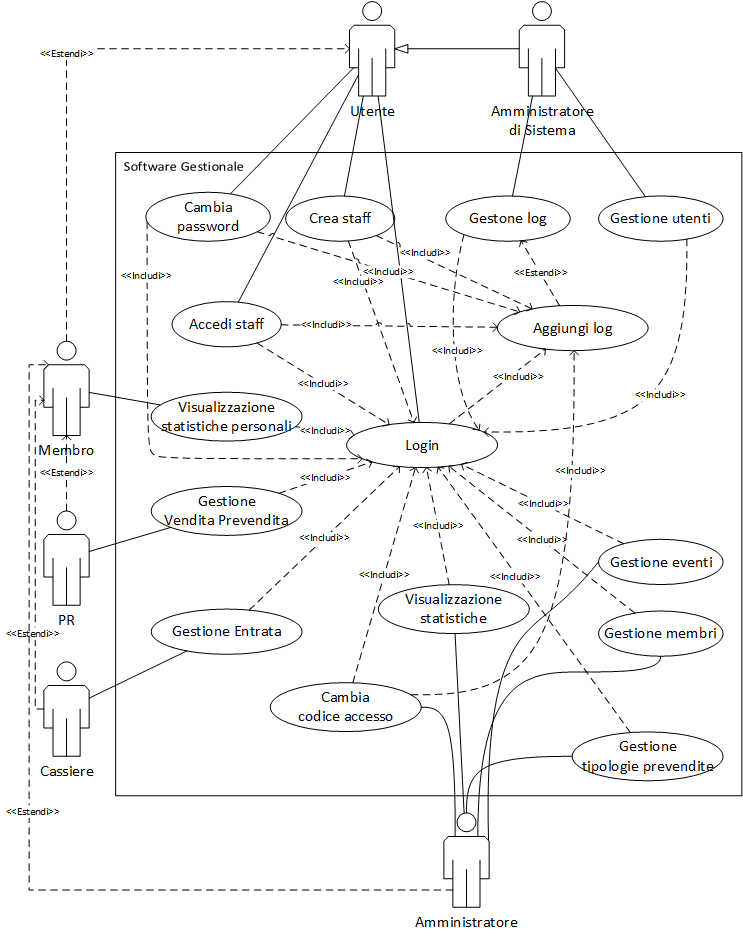
\includegraphics[scale=0.9]{use_cases.png}

L'utilizzo del login (frecce \textcolor{orange}{arancioni}) è necessario per tutti i servizi forniti agli attori.\\Con le frecce \textcolor{violet}{viola} abbiamo voluto evidenziare la maggior parte degli scenari che estendono la gestione degli utenti o dello staff.\\Abbiamo differenziato i casi d'uso delle statistiche perché si tratta di concetti diversi.    

\newpage

\subsubsection{Scenari}

%Login

\begin{center}
\begin{tabularx}{1\textwidth}{|l|X|}
    \hline
	\textbf{Titolo} & Login \\
	\hline
	\textbf{Descrizione} & Autenticazione nel software gestionale \\
	\hline
	\textbf{Attori} & Utente \\
	\hline
	\textbf{Relazioni} & Cambia Password \\
	\hline
	\textbf{Precondizioni} & L'utente deve essere registato nel sistema \\
	\hline
	\textbf{Postcondizioni} & L'utente è autenticato nel sistema \\
	\hline
	\textbf{Scenario principale} & 1. Impostazione di una schermata per l'inserimento di username e password. \\
								 & 2. L'utente inserisce i dati del proprio account. \\
								 & 3. L'utente esegue l'operazione. \\
								 & 4. Il sistema verifica le credenziali. \\
								 & 5. Dopo l'autenticazione viene mostrata una schermata principale.\\
	\hline
	\textbf{Scenari alternativi} & A) L'utente sbaglia credenziali: \\
								 & \quad 1. Notifica all'utente.\\
								 & \quad 2. Ritorno alla schermata di login.\\
								 & B) L'utente ha sbagliato troppe volte le credenziali: \\
								 & \quad 1. Blocco dell'account.\\
								 & \quad 2. Notifica all'utente.\\
								 & \quad 3. Ritorno alla schermata di login.\\
								 & C) L'utente ha la password di default impostata dall'amministratore di sistema:\\
								 & \quad 1. Passaggio al cambio password.\\
								 & D) L'utente ha l'account bloccato:\\
								 & \quad 1. Notifica all'utente.\\
								 & \quad 2. Ritorno alla schermata di login.\\
								 & E) L'utente è gia autenticato:\\
								 & \quad 1. Mostro la schermata principale.\\
	\hline
	\textbf{Requisiti non funzionali} & \hyperlink{R1NF}{R1NF}, \hyperlink{R6NF}{R6NF}, \hyperlink{R15NF}{R15NF} \\
	\hline
	\textbf{Punti aperti} & \\
	\hline
\end{tabularx}
\end{center}
  
%Gestione utente

\begin{center}
\begin{tabularx}{1\textwidth}{|l|X|}
    \hline
	\textbf{Titolo} & Gestione utente \\
	\hline
	\textbf{Descrizione} & Gestione degli utenti presenti nel software gestionale \\
	\hline
	\textbf{Attori} & Utente \\
	\hline
	%\textbf{Relazioni} & Login, Cambia password, Accedi staff, Crea staff, Gestione log, Registrazione utente, Sblocco utente \\
	\textbf{Relazioni} & Login, Cambia password, Accedi staff, Crea staff, Registrazione utente \\
	\hline
	\textbf{Precondizioni} &  \\
	\hline
	\textbf{Postcondizioni} &  \\
	\hline
	\textbf{Scenario principale} & 1. L'utente risulta già autenticato.\\
	                             & 2. Viene mostrata una schermata con le azioni possibili:\\
								 & \quad a. Cambia Password.\\
								 & \quad b. Accedi staff.\\
								 & \quad c. Crea staff.\\
								 & 2b. Se l'utente è anche amministratore di sistema, vengono aggiunte delle scelte:\\
								 %& \quad d. Gestione log.\\
								 & \quad e. Registrazione utente.\\
								 %& \quad f. Sblocco utente.\\
								 & 3. L'utente sceglie l'operazione desiderata.\\
								 & 4. Il sistema cambia vista a seconda della scelta.\\
	\hline
	\textbf{Scenari alternativi} & A) L'utente non è autenticato: \\
								 & \quad 1. Notifica all'utente.\\
								 & \quad 2. Passaggio al login.\\
	\hline
	\textbf{Requisiti non funzionali} & \\
	\hline
	\textbf{Punti aperti} & \\
	\hline
\end{tabularx}
\end{center}

%Qui metto i casi d'uso sotto gestione utente------------------------------------------

%Registrazione utente

\begin{center}
\begin{tabularx}{1\textwidth}{|l|X|}
    \hline
	\textbf{Titolo} & Registrazione utente \\
	\hline
	\textbf{Descrizione} & Una persona ha richiesto l'accesso al sistema gestionale e l'amministratore vuole registrarlo. \\
	\hline
	\textbf{Attori} & Amministratore di sistema, Utente \\
	\hline
	\textbf{Relazioni} & Gestione utente \\
	\hline
	\textbf{Precondizioni} &  \\
	\hline
	\textbf{Postcondizioni} &  \\
	\hline
	\textbf{Scenario principale} & 1. L'amministratore di sistema è già autenticato.\\
	                             & 2. L'amministratore si informa riguardo l'utente, chiedendo informazioni per la registrazione.\\
								 & 3. L'utente fornisce i dati all'amministratore.\\
								 & 4. L'amministratore sceglie username e password iniziale per l'utente, utilizzando criteri di sicurezza.\\
	\hline
	\textbf{Scenari alternativi} & A) Dati dell'utente da registrare in conflitto o non validi: \\
								 & \quad 1. Notifica all'amministratore.\\
								 & \quad 2. L'amministratore cerca di correggere i dati.\\
								 & \quad 3. L'amministratore ripete l'operazione.\\
	\hline
	\textbf{Requisiti non funzionali} & \hyperlink{R1NF}{R1NF} \\
	\hline
	\textbf{Punti aperti} & \\
	\hline
\end{tabularx}
\end{center}




%Aggiungi log
%Non so se mettere la relazione con login.

% \begin{center}
% \begin{tabularx}{1\textwidth}{l|X}
% \textbf{Titolo} & Aggiungi log \\
% \hline
% \textbf{Descrizione} & Aggiunta di una voce di log nel sistema gestionale \\
% \hline
% \textbf{Attori} & Amministratore di sistema \\
% \hline
% \textbf{Relazioni} & Gestione log \\
% \hline
% \textbf{Precondizioni} &  \\
% \hline
% \textbf{Postcondizioni} &  \\
% \hline
% \textbf{Scenario principale} & 1. Il sistema mostra una vista per l'inserimento della voce del log.\\
% & 2. L'amministratore di sistema aggiunge le informazioni.\\
% & 3. L'amministratore esegue l'operazione.\\
% & 4. Ritorno alla schermata precedente.\\
% \hline
% \textbf{Scenari alternativi} & A) L'utente non è autenticato: \\
% & \quad 1. Notifica all'utente.\\
% & \quad 2. Passaggio al login.\\
% & B) L'utente non è amministratore di sistema:\\
% & \quad 1. Notifica all'utente.\\
% & \quad 2. Passaggio alla schermata precedente.\\
% & C) La richiesta di aggiunta log viene

% \hline
% \textbf{Requisiti non funzionali} &  \hyperlink{R21NF}{R21NF} \\
% \hline
% \textbf{Punti aperti} & \\
% \hline
% \end{tabularx}
% \end{center}

% Crea staff

\begin{center}
\begin{tabularx}{1\textwidth}{|l|X|}
    \hline
		\textbf{Titolo} & Crea staff \\
		\hline
		\textbf{Descrizione} & Creazione di uno staff \\
		\hline
		\textbf{Attori} & Utente \\
		\hline
		\textbf{Relazioni} & Gestione utente \\
		\hline
		\textbf{Precondizioni} &  \\
		\hline
		\textbf{Postcondizioni} &  \\
		\hline
		\textbf{Scenario principale} & 1. L'utente è già autenticato.\\
		                             & 2. L'utente accede alla creazione staff. \\
									 & 3. Il sistema fornisce una vista di creazione. \\
									 & 4. L'utente inserisce i dati del nuovo staff. \\
									 & 5. L'utente esegue l'operazione.\\
									 & 6. Ritorno alla schermata precedente.\\
		\hline
		\textbf{Scenari alternativi} & A) L'utente ha già creato uno staff: \\
									 & \quad 1. Notifica all'utente \\
									 & \quad 2. Ritorno alla schermata precedente.\\
		\hline
		\textbf{Requisiti non funzionali} & \hyperlink{R2NF}{R2NF} \\
		\hline
		\textbf{Punti aperti} & \\
		\hline
	\end{tabularx}
\end{center}

%Cambia password

\begin{center}
\begin{tabularx}{1\textwidth}{|l|X|}
    \hline
	\textbf{Titolo} & Cambia password \\
	\hline
	\textbf{Descrizione} & Cambio della password di un utente \\
	\hline
	\textbf{Attori} & Utente \\
	\hline
	\textbf{Relazioni} & Gestione utente \\
	\hline
	\textbf{Precondizioni} &  \\
	\hline
	\textbf{Postcondizioni} &  \\
	\hline
	\textbf{Scenario principale} & 1. L'utente è già autenticato.\\
	                             & 2. L'utente accede al cambio password. \\
								 & 3. Il sistema fornisce una vista. \\
								 & 4. L'utente inserisce i dati per il cambio di password. \\
								 & 5. L'utente esegue l'operazione.\\
								 & 6. Ritorno alla schermata precedente.\\
	\hline
	\textbf{Scenari alternativi} & \\
	\hline
	\textbf{Requisiti non funzionali} & \hyperlink{R1NF}{R1NF} \\
	\hline
	\textbf{Punti aperti} & \\
	\hline
\end{tabularx}
\end{center}

%Accedi staff

\begin{center}
\begin{tabularx}{1\textwidth}{|l|X|}
    \hline
	\textbf{Titolo} & Accedi allo staff \\
	\hline
	\textbf{Descrizione} & Permettere di diventare membro di uno staff \\
	\hline
	\textbf{Attori} & Utente \\
	\hline
	\textbf{Relazioni} & Gestione utente\\
	\hline
	\textbf{Precondizioni} &  \\
	\hline
	\textbf{Postcondizioni} &  \\
	\hline
	\textbf{Scenario principale} & 1. L'utente è già autenticato.\\
	                             & 2. L'utente accede alla schermata di accedi staff. \\
								 & 3. Il sistema fornisce una vista. \\
								 & 4. L'utente inserisce i dati per l'accesso allo staff. \\
								 & 5. L'utente esegue l'operazione.\\
								 & 6. Ritorno alla schermata precedente.\\
	\hline
	\textbf{Scenari alternativi} & A) L'utente è già membro dello staff:\\
								 & \quad 1. Notifica all'utente.\\
								 & \quad 2. Ritorno alla schermata precedente.\\
								 & B) L'utente ha fornito un codice di accesso errato:\\
								 & \quad 1. Notifica all'utente.\\
	\hline
	\textbf{Requisiti non funzionali} & \hyperlink{R2NF}{R2NF} \\
	\hline
	\textbf{Punti aperti} & \\
	\hline
\end{tabularx}
\end{center}

%----------------------------------------------------------------------------------------

%Gestione staff

\begin{center}
\begin{tabularx}{1\textwidth}{|l|X|}
    \hline
	\textbf{Titolo} & Gestione staff \\
	\hline
	\textbf{Descrizione} & Gestione dello staff dell'utente \\
	\hline
	\textbf{Attori} & Membro \\
	\hline
	\textbf{Relazioni} & Login, Visualizzazione statistiche personali, Gestione vendita prevendita, Gestione entrata, Gestione membri, Cambia codice di accesso, Visualizzazione statistiche, Gestione eventi, Gestione tipologie prevendite \\
	\hline
	\textbf{Precondizioni} & \\
	\hline
	\textbf{Postcondizioni} & \\
	\hline
	\textbf{Scenario principale} & 1. Il membro è già autenticato.\\
	                             & 2. Viene mostrata una schermata con le azioni possibili:\\
								 & \quad a. Visualizza statistiche personali.\\
								 & 2b. Se il membro è anche PR dello staff, vengono aggiunte delle scelte:\\
								 & \quad b. Gestione vendita prevendita.\\
								 & 2c. Se il membro è anche cassiere dello staff, vengono aggiunte delle scelte:\\
								 & \quad c. Gestione entrata.\\
								 & 2d. Se il membro è anche amministratore dello staff, vengono aggiunte delle scelte:\\
								 & \quad d. Gestione membri.\\
								 & \quad d. Cambia codice di accesso.\\
								 & \quad d. Visualizzazione statistiche.\\
								 & \quad d. Gestione eventi.\\
								 & \quad d. Gestione tipologie prevendite.\\
								 & 3. il membro sceglie l'operazione desiderata.\\
								 & 4. Il sistema cambia vista a seconda della scelta.\\
	\hline
	\textbf{Scenari alternativi} & \\
	\hline
	\textbf{Requisiti non funzionali} & \\
	\hline
	\textbf{Punti aperti} & \\
	\hline
\end{tabularx}
\end{center}
  
%Qui metto i casi d'uso sotto gestione staff--------------------------------------------------

%Visualizza statistiche personali

\begin{center}
\begin{tabularx}{1\textwidth}{|l|X|}
    \hline
	\textbf{Titolo} & Visualizza statistiche personali \\
	\hline
	\textbf{Descrizione} & Permettere di visualizzare le statistiche personali di un membro come PR o cassiere. \\
						 & Non è associato direttamente a PR e a cassiere perché i ruoli di un membro potrebbero cambiare.\\
	\hline
	\textbf{Attori} & Membro \\
	\hline
	\textbf{Relazioni} & Gestione staff \\
	\hline
	\textbf{Precondizioni} &  \\
	\hline
	\textbf{Postcondizioni} &  \\
	\hline
	\textbf{Scenario principale} & 1. Il membro è già autenticato.\\
	                             & 2. Il membro accede alla schermata di vusualizzazione delle statistiche personali.\\
								 & 3. Il sistema fornisce una vista con tutte le statistiche. \\
								 & 4. Quando il membro ha finito la consultazione, ritorna alla schermata precedente.\\
	\hline
	\textbf{Scenari alternativi} & \\
	\hline
	\textbf{Requisiti non funzionali} & \\
	\hline
	\textbf{Punti aperti} & \\
	\hline
\end{tabularx}
\end{center}

%Gestione vendita prevendita: aggiungi prevendita, annulla prevendita

\begin{center}
\begin{tabularx}{1\textwidth}{|l|X|}
    \hline
	\textbf{Titolo} & Gestione vendita prevendita \\
	\hline
	\textbf{Descrizione} & Permette di gestire la vendita di una prevendita: aggiunta prevendita, annulla prevendita \\
	\hline
	\textbf{Attori} & PR, Cliente \\
	\hline
	\textbf{Relazioni} & Gestione staff \\
	\hline
	\textbf{Precondizioni} &  \\
	\hline
	\textbf{Postcondizioni} &  \\
	\hline
	\textbf{Scenario principale} & 1. Il PR è già autenticato.\\
	                             & 2. Il PR accede alla schermata di gestione prevenite. \\
								 & 3. Il sistema fornisce una vista con le opzioni possibili. \\
								 & 4. Il PR sceglie l'operazione:\\
								 & \quad a. Aggiungi prevendita.\\
								 & \quad b. Annulla prevendita.\\
								 & \quad c. Lista prevendite.\\
								 & 5. Il PR inserisce i dati relativi all'operazione, consultando il cliente se necessario.\\
								 & 6. Il PR esegue l'operazione.\\
								 & 7bis. Nel caso di aggiungi prevendita si consegna al cliente il documento digitale.\\
								 & 8. Ritorno alla schermata precedente.\\
	\hline
	\textbf{Scenari alternativi} & \\
	\hline
	\textbf{Requisiti non funzionali} & \hyperlink{R7NF}{R7NF}, \hyperlink{R8NF}{R8NF}, \hyperlink{R9NF}{R9NF}, \hyperlink{R11NF}{R11NF}, \hyperlink{R13NF}{R13NF}, \hyperlink{R14NF}{R14NF}, \hyperlink{R16NF}{R16NF}, \hyperlink{R18NF}{R18NF}  \\
	\hline
	\textbf{Punti aperti} & \\
	\hline
\end{tabularx}
\end{center}

%Gestione entrata: timbra entrata, leggi prevendita,

\begin{center}
\begin{tabularx}{1\textwidth}{|l|X|}
    \hline
	\textbf{Titolo} & Gestione entrata \\
	\hline
	\textbf{Descrizione} & Permette di gestire l'entrata di un cliente: timbratura dell'entrata \\
	\hline
	\textbf{Attori} & Cassiere, Cliente \\
	\hline
	\textbf{Relazioni} & Gestone staff \\
	\hline
	\textbf{Precondizioni} &  \\
	\hline
	\textbf{Postcondizioni} &  \\
	\hline
	\textbf{Scenario principale} & 1. Il Cassiere è già autenticato.\\
	                             & 2. Il Cassiere accede alla schermata di gestione entrata. \\
								 & 3. Il sistema fornisce una vista con le opzioni disponibile.\\
								 & 4. Il Cassiere sceglie l'operazione:\\
								 & \quad a.Timbra entrata.\\
								 & \quad b. Lista entrate.\\
								 & 5. Il Cassiere inserisce i dati dell'operazione, consultando il cliente se necessario.\\
								 & 6. Il cassiere esegue l'operazione.\\
								 & 7. Il Cassiere informa il cliente riguardo l'esito dell'operazione, se necessario.\\
								 & 8. Ritorno alla schermata precedente.\\
	\hline
	\textbf{Scenari alternativi} & \\
	\hline
	\textbf{Requisiti non funzionali} & \hyperlink{R17NF}{R17NF}, \hyperlink{R19NF}{R19NF} \\
	\hline
	\textbf{Punti aperti} & \\
	\hline
\end{tabularx}
\end{center}


%Cambia codice accesso

\begin{center}
\begin{tabularx}{1\textwidth}{|l|X|}
    \hline
	\textbf{Titolo} & Cambia codice accesso \\
	\hline
	\textbf{Descrizione} & Cambio del codice di accesso allo staff \\
	\hline
	\textbf{Attori} & Amministratore \\
	\hline
	\textbf{Relazioni} & Gestone staff \\
	\hline
	\textbf{Precondizioni} &  \\
	\hline
	\textbf{Postcondizioni} &  \\
	\hline
	\textbf{Scenario principale} & 1. L'amministratore è già autenticato.\\
	                             & 2. L'amministratore accede al cambio codice di accesso. \\
								 & 3. Il sistema fornisce una vista. \\
								 & 4. L'amministratore inserisce i dati per il cambio del codice. \\
								 & 5. L'amministratore esegue l'operazione.\\
								 & 6. Ritorno alla schermata precedente.\\
	\hline
	\textbf{Scenari alternativi} & \\
	\hline
	\textbf{Requisiti non funzionali} & \hyperlink{R2NF}{R2NF} \\
	\hline
	\textbf{Punti aperti} & \\
	\hline
\end{tabularx}
\end{center}

%Visualizza statistiche 

\begin{center}
\begin{tabularx}{1\textwidth}{|l|X|}
    \hline
	\textbf{Titolo} & Visualizza statistiche \\
	\hline
	\textbf{Descrizione} & Permettere di visualizzare le statistiche dello staff. \\
	\hline
	\textbf{Attori} & Amministratore \\
	\hline
	\textbf{Relazioni} & Gestone staff \\
	\hline
	\textbf{Precondizioni} &  \\
	\hline
	\textbf{Postcondizioni} &  \\
	\hline
	\textbf{Scenario principale} & 1. L'amministratore è già autenticato.\\
	                             & 2. L'amministratore accede alla schermata di vusualizzazione. \\
								 & 3. Il sistema fornisce una vista con tutte le statistiche. \\
								 & 4. Quando l'amministratore ha finito la consultazione, ritorna alla schermata precedente.\\
	\hline
	\textbf{Scenari alternativi} & \\
	\hline
	\textbf{Requisiti non funzionali} & \hyperlink{R5NF}{R5NF} \\
	\hline
	\textbf{Punti aperti} & \\
	\hline
\end{tabularx}
\end{center}

%Gestione eventi: aggiungi evento, modifica evento, annulla evento

\begin{center}
\begin{tabularx}{1\textwidth}{|l|X|}
    \hline
	\textbf{Titolo} & Gestione eventi \\
	\hline
	\textbf{Descrizione} & Permettere di gestire gli eventi dello staff. \\
	\hline
	\textbf{Attori} & Amministratore \\
	\hline
	\textbf{Relazioni} & Gestone staff \\
	\hline
	\textbf{Precondizioni} &  \\
	\hline
	\textbf{Postcondizioni} &  \\
	\hline
	\textbf{Scenario principale} & 1. L'amministratore è già autenticato.\\
	                             & 2. L'amministratore accede alla schermata di vusualizzazione. \\
								 & 3. Il sistema fornisce una vista con le scelte: \\
								 & \quad a. Aggiungi evento.\\
								 & \quad b. Modifica evento.\\
								 & \quad c. Annulla evento.\\
								 & \quad d. Lista eventi.\\
								 & 4. Una volta scelta l'operazione, l'amministratore inserisce i dati richiesti. \\
								 & 5. L'amministratore esegue l'operazione.\\
								 & 6. Ritorno alla schermata precedente.\\
	\hline
	\textbf{Scenari alternativi} & \\
	\hline
	\textbf{Requisiti non funzionali} & \hyperlink{R7NF}{R7NF}, \hyperlink{R10NF}{R10NF} \\
	\hline
	\textbf{Punti aperti} & \\
	\hline
\end{tabularx}
\end{center}

%Gestione tipologie prevendite: aggiungi tipologia prevendita, modifica tipologia prevendita, elimina tipologia prevendita.

\begin{center}
\begin{tabularx}{1\textwidth}{|l|X|}
    \hline
	\textbf{Titolo} & Gestione tipologie prevendite \\
	\hline
	\textbf{Descrizione} & Permettere di gestire le tipologie associate alle prevendite di un evento. \\
	\hline
	\textbf{Attori} & Amministratore \\
	\hline
	\textbf{Relazioni} & Gestone staff \\
	\hline
	\textbf{Precondizioni} &  \\
	\hline
	\textbf{Postcondizioni} &  \\
	\hline
	\textbf{Scenario principale} & 1. L'amministratore è già autenticato.\\
	                             & 2. L'amministratore accede alla schermata di vusualizzazione. \\
								 & 3. Il sistema fornisce una vista con le scelte: \\
								 & \quad a. Aggiungi tipologia evento.\\
								 & \quad b. Modifica tipologia evento.\\
								 & \quad c. Elimina tipologia evento.\\
								 & \quad d. Lista tipologie evento.\\
								 & 4. Una volta scelta l'operazione, l'amministratore inserisce i dati richiesti. \\
								 & 5. L'amministratore esegue l'operazione.\\
								 & 6. Ritorno alla schermata precedente.\\
	\hline
	\textbf{Scenari alternativi} & \\
	\hline
	\textbf{Requisiti non funzionali} & \hyperlink{R8NF}{R8NF}, \hyperlink{R15NF}{R15NF} \\
	\hline
	\textbf{Punti aperti} & \\
	\hline
\end{tabularx}
\end{center}

%Gestione membri: modifica diritti membro, rimuovi membro

\begin{center}
\begin{tabularx}{1\textwidth}{|l|X|}
    \hline
	\textbf{Titolo} & Gestione membri \\
	\hline
	\textbf{Descrizione} & Permettere di gestire i membri dello staff, concedendo i ruoli o rimuovendo i membri. \\
	\hline
	\textbf{Attori} & Amministratore \\
	\hline
	\textbf{Relazioni} & Gestone staff \\
	\hline
	\textbf{Precondizioni} &  \\
	\hline
	\textbf{Postcondizioni} &  \\
	\hline
	\textbf{Scenario principale} & 1. L'amministratore è già autenticato.\\
	                             & 2. L'amministratore accede alla schermata di vusualizzazione. \\
								 & 3. Il sistema fornisce una vista con le scelte: \\
								 & \quad a. Modifica ruoli membro.\\
								 & \quad b. Rimuovi membro.\\
								 & \quad c. Lista membri.\\
								 & 4. Una volta scelta l'operazione, l'amministratore inserisce i dati richiesti. \\
								 & 5. L'amministratore esegue l'operazione.\\
								 & 6. Ritorno alla schermata precedente.\\
	\hline
	\textbf{Scenari alternativi} & A) L'amministratore si vuole rimuovere ma è l'unico amministratore rimasto nello staff: \\
								 & \quad 1. Notifica all'utente. \\
								 & \quad 2. Ritorno alla schermata precedente. \\
	\hline
	\textbf{Requisiti non funzionali} & \hyperlink{R16F/NF}{R16F/NF} \\
	\hline
	\textbf{Punti aperti} & \\
	\hline
\end{tabularx}
\end{center}

%------------------------------------------------------------------------------------------

\newpage

\subsection{Analisi del rischio}

%Alla fine di questa parte vanno introdotti i seguenti vincoli:
%Log delle operazioni
%Blocco utente dopo un tot di tentativi
%Cifratura della comunicazione
%Sistema anti contraffazione: prevendita nominativa + codice
%Sistema locale durante l'evento

\subsubsection{Valutazione dei beni}

\begin{center}
    \begin{tabularx}{1\textwidth}{|X|X|X|}
         \hline
         \textbf{Bene} & \textbf{Valore} & \textbf{Esposizione}  \\
         \hline
         \hline
         Sistema gestionale & Alto & Alta \\
                            & Registra tutte le prevendite di uno staff. Critico dal punto di vista della sicurezza & Perdita d'immagine del software e degli staff, spesa in tempo per il ripristino del backup, se il sistema fallisce è necessario acquistare prevendite fisiche. Possibili perdite finanziare \\
         \hline
         Informazioni su utenti & Medio-Alto & Alta\\
                            & Informazioni relative agli utenti del sistema, anche le credenziali, le quali potrebbero permettere l'accesso ai dati dello staff e relativi clienti & Perdita d'immagine del software, un membro con ruolo amministrativo potrebbe compromettere temporaneamente uno staff fino a ripristino backup. Possibile perdita economica dovuta all'aggiunta di prevendite.\\
         \hline
         Informazioni su prevendite & Alto & Alta \\
                                    & Rappresentano i guadagni per uno staff, nonché il biglietto d'ingresso di un cliente & Perdita d'immagine del software: lo staff ha perso informazioni riguardo i ricavi, perdita d'immagine dello staff: il cliente non riesce a entrare. Possibile perdita economica se vengono aggiunte prevendite non dovute.\\
         \hline
         Informazioni su clienti & Medio & Bassa \\
                                  & Le informazioni sono ridotte al solo nome e cognome (\hyperlink{R25F}{R25F}) & \\
         \hline
         Informazioni su amministratori di sistema & Medio-Alto &  Alta \\
                                                    & Hanno lo stesso valore di quelle degli utenti & Tutte le esposizioni sulle informazioni degli utenti, più la possibilità di perdere log\\ 
         \hline
    \end{tabularx}
\end{center}

\subsubsection{Analisi minacce e controlli}


\begin{center}
    \begin{tabulary}{1\textwidth}{|L|C|C|C|}
        \hline
        \textbf{Minaccia} & \textbf{Probabilità} & \textbf{Controllo} & \textbf{Fattibilità}  \\
        \hline
        \hline
        Furto d’identità (utente) & Media-Bassa. Username e password scelti dall'amministratore di sistema & Log degli accessi, blocco dell'utente & Costo minimo\\
        \hline
        Furto d’identità (amministratore di sistema) & Bassa & Log degli accessi & Costo minimo\\
        \hline
        Alterazione dei dati nella comunicazione & Medio-Alta. Molte comunicazione avvengono nel sistema distribuito client/server. & Uso di canale sicuro & Costo basso anche se si utilizza un mix tra chiave simmetrica e asimmetrica\\
        Man in the Middle &  &  & \\
        \hline
        %DoS/DDoS & Bassa & Sistema locale durante l'evento (\hyperlink{R19NF}{R19NF}) & Costo medio, richiesta di risorse hardware portatili\\
        DoS/DDoS & Bassa & Sistema locale durante l'evento & Costo medio, richiesta di risorse hardware portatili\\
        \hline
        %Contraffazione della prevendita & Alta & Sistema anti-contraffazione (\hyperlink{R20NF}{R20NF}), prevendita nominativa & Costo minimo\\
        Contraffazione della prevendita & Alta & Sistema anti-contraffazione, prevendita nominativa & Costo minimo\\
        \hline
        Furto della prevendita & Media & prevendita nominativa & Costo minimo\\
        \hline
    \end{tabulary}
\end{center}

\newpage

\subsubsection{Analisi della tecnologia dal punto di vista della sicurezza}

\begin{center}
    \begin{tabulary}{1\textwidth}{|L|C|}
        \hline
        \textbf{Tecnologia} & \textbf{Vulnerabilità} \\
        \hline
        \hline
        Cifratura delle comunicazioni & Utilizzo di una doppia cifratura simmetrica+asimmetrica con le loro relative vulnerabilità.\\
                                      & L'utilizzo di cifrature standard potrebbero causare vulnerabilià ulteriori.\\
        \hline
        Autenticazione tramite credenziali & Social engineering \\
                                           & Password cracking \\
                                           & Negligenza \\
        \hline
        Architettura Client/Server & Attacco DDoS/DoS \\
                                   & Attacco Man in the Middle\\
                                   & Sniffing della comunicazione\\
                                   & Deadlock\\
                                   & Esposizione dei client\\
        \hline
        %Non so se questa va bene.
        %Servizio di hosting esterno & Esposizione dei dati \\
        %\hline
    \end{tabulary}
\end{center}

\subsubsection{Security Use Case e Misuse Case}

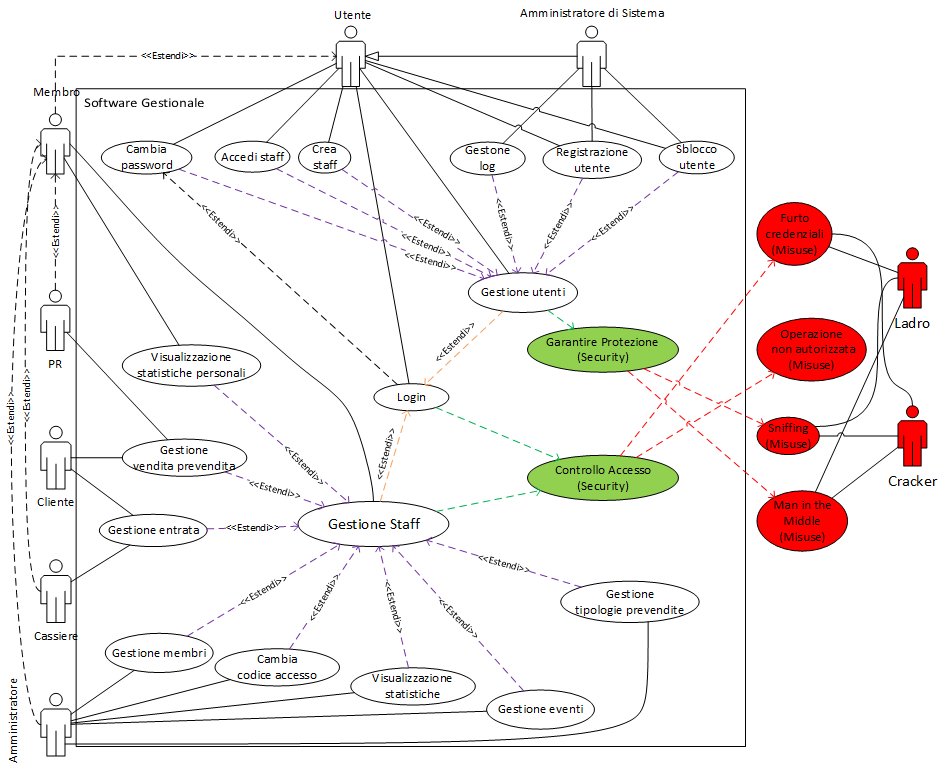
\includegraphics[scale=0.73]{security_use_cases_misuse_cases.png}

\newpage

\begin{center}
\begin{tabularx}{1\textwidth}{|X|X|X|}
    \hline
    \textbf{Caso d’uso} & \mc{2}{Garantire Protezione}\\
    \hline
    \textbf{Percorso d’uso} & \mc{2}{Garantire Protezione dei dati persistenti}\\
    \hline
    \textbf{Misuse case} & \mc{2}{Man in the Middle, Sniffing, Furto credenziali}\\
    \hline
    \textbf{Descrizione} & \mc{2}{I dati persistenti devono essere protetti.}\\
    \hline
    \textbf{Rischi alla sicurezza} & \mc{2}{Un utente malintenzionato potrebbe modificare o compromettere i dati relativi al software gestionale, come i gli utenti registrati o le prevendite di un evento.}\\
    \hline
    \textbf{Precondizioni} & \mc{2}{ 1. Il sistema è già stato utilizzato dall'amministratore di sistema per la registrazione degli utenti e/o uno staff ha già registrato delle prevendite per un evento.}\\
    & \mc{2}{2. L'attaccante ha i mezzi necessari per tentare di modificare i dati persistenti.}\\
    \hline
    \textbf{Postcondizioni} & \mc{2}{ Il sistema blocca il tentativo di modifica o compromissione dei dati persistenti.}\\
    \hline
    \textbf{Scenario principale} & \textbf{Sistema} & \textbf{Attaccante}\\
    \hline
    & & L'attaccante cerca di modificare dati persistenti del sistema gestionale \\
    \cline{2-3}
    & Il sistema blocca l'attacco e notifica l'amministratore di sistema.  &  \\
    \hline
    \textbf{Scenario di attacco avvenuto con successo} & \textbf{Sistema} & \textbf{Attaccante}\\
    \hline
    & & L'attaccante riesce ad accedere/modificare dati persistenti\\
    \cline{2-3}
    & Il sistema registra nei log le modifiche effettuate & \\
    \cline{2-3}
    & L'amministratore di sistema nota i log anomali e opera di conseguenza & \\
    \hline
\end{tabularx}
\end{center}

\begin{center}
\begin{tabularx}{1\textwidth}{|X|X|X|}
    \hline
    \textbf{Caso d’uso} & \mc{2}{Garantire Protezione}\\
    \hline
    \textbf{Percorso d’uso} & \mc{2}{Garantire Protezione dei dati della comunicazione}\\
    \hline
    \textbf{Misuse case} & \mc{2}{Man in the Middle, Sniffing, Furto credenziali}\\
    \hline
    \textbf{Descrizione} & \mc{2}{I dati che viaggiano nelle comunicazioni devono essere protetti.}\\
    \hline
    \textbf{Rischi alla sicurezza} & \mc{2}{Un utente malintenzionato potrebbe leggere o alterare i dati in transito in una comunicazione.}\\
    \hline
    \textbf{Precondizioni} & \mc{2}{1. Il malintezionato ha la possibilità di intercettare i dati.}\\
    & \mc{2}{2. Il malintenzionato ha la possibilità di modificare i dati.}\\
    & \mc{2}{3. ha i mezzi per spedire il messaggio modificato al destinatario.}\\
    \hline
    \textbf{Postcondizioni} & \mc{2}{ Il sistema rileva il tentativo di modifica della comunicazione.}\\
    \hline
    \textbf{Scenario principale} & \textbf{Sistema} & \textbf{Attaccante}\\
    \hline
    & Il sistema si occupa di garantire una comunicazione dei messaggi sicura. & \\
    \cline{2-3}
    & & L'attaccante rileva un messaggio in transito, lo interecetta, lo modifica e lo inoltra all'utente finale. \\
    \cline{2-3}
    & Il sistema riceve il messaggio modificato e rileva il tentativo di lettura o modifca, rifiutandolo e segnalandolo nei log.  &  \\
    \hline
    \textbf{Scenario di attacco avvenuto con successo} & \textbf{Sistema} & \textbf{Attaccante}\\
    \hline
    & Il sistema si occupa di garantire una comunicazione dei messaggi sicura. & \\
    \cline{2-3}
    & & L'attaccante riesce ad alterare la comunicazione senza che il sistema se ne accorga.\\
    \cline{2-3}
    & Il sistema registra nei log le modifiche effettuate. & \\
    \cline{2-3}
    & L'amministratore di sistema nota i log anomali e opera di conseguenza. & \\
    \hline
\end{tabularx}
\end{center}

\begin{center}
\begin{tabularx}{1\textwidth}{|X|X|X|}
    \hline
    \textbf{Caso d’uso} & \mc{2}{Garantire Protezione}\\
    \hline
    \textbf{Percorso d’uso} & \mc{2}{Garantire Protezione rispetto alle contraffazioni}\\
    \hline
    \textbf{Misuse case} & \mc{2}{Contraffazione}\\
    \hline
    \textbf{Descrizione} & \mc{2}{Devo garantire che le prevendite lette siano autentiche.}\\
    \hline
    \textbf{Rischi alla sicurezza} & \mc{2}{Un utente malintenzionato potrebbe falsificare una prevendita.}\\
    \hline
    \textbf{Precondizioni} & \mc{2}{1. Il malintezionato conosce la struttura di una prevendita.}\\
    & \mc{2}{2. Il malintenzionato ha la possibilità di falsificare la prevendita.}\\
    \hline
    \textbf{Postcondizioni} & \mc{2}{ Il sistema rileva che la prevendita non è autentica.}\\
    \hline
    \textbf{Scenario principale} & \textbf{Sistema} & \textbf{Attaccante}\\
    \hline
    & Il sistema si occupa di garantire l'autenticità delle prevendite consegnate. & \\
    \cline{2-3}
    & & L'attaccante crea una prevendita falsificata e tenta il riconoscimento da parte del sistema. \\
    \cline{2-3}
    & Il sistema rileva che la prevendita è contraffatta, rifiutandola e segnalandola nei log.  &  \\
    \hline
    \textbf{Scenario di attacco avvenuto con successo} & \textbf{Sistema} & \textbf{Attaccante}\\
    \hline
    & Il sistema si occupa di garantire l'autenticità delle prevendite consegnate. & \\
    \cline{2-3}
    & & L'attaccante riesce a creare una prevendita che illuda il sistema.\\
    \cline{2-3}
    & Il sistema registra nei log l'entrata effettuata. & \\
    \cline{2-3}
    & L'amministratore dello staff nota una discrepanza e informa l'amministratore di sistema. & \\
    \cline{2-3}
    & L'amministratore di sistema fa una ricerca nei log e tenta di risalire al malfattore. & \\
    \hline
\end{tabularx}
\end{center}

\begin{center}
\begin{tabularx}{1\textwidth}{|X|X|X|}
    \hline
    \textbf{Caso d’uso} & \mc{2}{Controllo Accesso}\\
    \hline
    \textbf{Percorso d’uso} & \mc{2}{Controllo sull'autenticazione dell'utente}\\
    \hline
    \textbf{Misuse case} & \mc{2}{Furto credenziali}\\
    \hline
    \textbf{Descrizione} & \mc{2}{Il sistema deve proteggere l'utente da intrusioni di malintenzionati}\\
    \hline
    \textbf{Rischi alla sicurezza} & \mc{2}{Un malintenzionato ruba i dati di identificazione e autenticazione ad un utente.}\\
    \hline
    \textbf{Precondizioni} & \mc{2}{1. Il malintezionato ha la possibilità di trovare l'username.}\\
    & \mc{2}{2. Il malintenzionato ha la possibilità di tentare l'accesso al sistema.}\\
    \hline
    \textbf{Postcondizioni} & \mc{2}{ Il sistema rileva il tentativo di accesso fraudolento e blocca l'utente.}\\
    \hline
    \textbf{Scenario principale} & \textbf{Sistema} & \textbf{Attaccante}\\
    \hline
    & & L'attaccante tenta un attacco di password cracking. \\
    \cline{2-3}
    & Il sistema rileva l'attacco e blocca l'account dell'utente. &  \\
    \hline
    \textbf{Scenario di attacco avvenuto con successo} & \textbf{Sistema} & \textbf{Attaccante}\\
    \hline
    & & L'attaccante riesce a scoprire la password \\
    \cline{2-3}
    & Il sistema fornisce l'accesso al sistema. & \\
    \cline{2-3}
    & & Il malintenzionato tenta di reperire tutte le informazioni prima di essere scoperto. \\
    \cline{2-3}
    & Il sistema notifica nei log le operazioni effettuate. & \\
    \cline{2-3}
    & L'amministratore di sistema nota i log anomali e opera di conseguenza. & \\
    \hline
\end{tabularx}
\end{center}

\begin{center}
\begin{tabularx}{1\textwidth}{|X|X|X|}
    \hline
    \textbf{Caso d’uso} & \mc{2}{Controllo Accesso}\\
    \hline
    \textbf{Percorso d’uso} & \mc{2}{Controllo sulle operazioni eseguite dagli utenti}\\
    \hline
    \textbf{Misuse case} & \mc{2}{Operazione non autorizzata}\\
    \hline
    \textbf{Descrizione} & \mc{2}{Il sistema deve evitare che utenti non autorizzati possano eseguire operazioni non concesse. Deve essere valido sia per i ruoli di uno staff, sia per il ruolo di amministratore di sistema.}\\
    \hline
    \textbf{Rischi alla sicurezza} & \mc{2}{Un utente normale esegue senza autorizzazione operazioni riservate all'amministratore di sistema.}\\
    & \mc{2}{Un membro di uno staff esegue senza autorizzazione operazioni riservate ad un ruolo che non ha.}\\
    \hline
    \textbf{Precondizioni} & \mc{2}{1. L'utente ha credenziali validi per l'accesso.}\\
    & \mc{2}{2. L'utente non ha i privilegi per cui sta tentando di effettuare l'operazione.}\\
    \hline
    \textbf{Postcondizioni} & \mc{2}{ Il sistema rileva il tentativo di esecuzione non autorizzata e blocca l'operazione.}\\
    \hline
    \textbf{Scenario principale} & \textbf{Sistema} & \textbf{Attaccante}\\
    \hline
    & & L'utente tenta di eseguire un operazione non consentita. \\
    \cline{2-3}
    & Il sistema verifica le autorizzazioni dell'utente e blocca l'operazione non autorizzata. &  \\
    & Il sistema aggiunge un record di log su quanto accaduto. &  \\
    \hline
\end{tabularx}
\end{center}

\begin{center}
\begin{tabularx}{1\textwidth}{|X|X|X|}
    \hline
    \textbf{Caso d’uso} & \mc{2}{Disponibilità}\\
    \hline
    \textbf{Misuse case} & \mc{2}{DDoS/DoS}\\
    \hline
    \textbf{Descrizione} & \mc{2}{Il sistema deve cercare di proteggersi da attacchi DDoS/DoS}\\
    \hline
    \textbf{Rischi alla sicurezza} & \mc{2}{Un malintenzionato vuole impedire l'accesso al sistema durante un evento.}\\
    \hline
    \textbf{Precondizioni} & \mc{2}{1. Il malintezionato dispone dei mezzi per effettuare l'attacco.}\\
    \hline
    \textbf{Postcondizioni} & \mc{2}{ Il sistema si protegge dalla minaccia.}\\
    \hline
    \textbf{Scenario principale} & \textbf{Sistema} & \textbf{Attaccante}\\
    \hline
    & & L'attaccante tenta un attacco DDoS/DoS. \\
    \cline{2-3}
    & Il sistema rileva l'attacco e informa l'amministratore di sistema, mentre cerca di attuare misure per ridurre l'efficacia dell'attacco. &  \\
    \cline{2-3}
    & Il sistema riesce a contenere l'attacco, dato che l'attaccante non ha sufficiente potenza per mettere fuori uso il sistema. &  \\
    \cline{2-3}
    & L'amministratore di sistema controlla lo stato e agisce di conseguenza. &  \\
    \hline
    \textbf{Scenario di attacco avvenuto con successo} & \textbf{Sistema} & \textbf{Attaccante}\\
    \hline
    & & L'attaccante tenta un attacco DDoS/DoS. \\
    \cline{2-3}
    & Il sistema rileva l’attacco e informal’amministratore di sistema, mentrecerca di attuare misure per ridurrel’efficacia dell’attacco. & \\
    \cline{2-3}
    & Il sistema non riesce a contenere l'attacco e va fuori uso. & \\
    \cline{2-3}
    & L'amministratore di sistema vede che il sistema di fuori uso e tenta un ripristino locale per favorire l'accesso al sistema durante l'evento. & \\
    \hline
\end{tabularx}
\end{center}

\subsubsection{Requisiti di Protezione dei Dati}

Dall’analisi del rischio sono emersi altri requisiti riguardanti la protezione dei dati:

\begin{itemize}
    \item Crazione di un sistema di log per il tracciamento delle operazioni svolte nel sistema gestionale, garantendo la persistenza dei log. L'amministratore di sistema è l'unico a poter accedere ai log. Per evitare l'uscita di informazioni riservate, cercare di memorizzare nei log solo le informazioni utili per l'analisi da parte dell'amministratore.
    \item Creare un sistema per il blocco dell'utente dopo un certo numero di tentativi. L'amministratore di sistema ha la possibilità di sbloccare l'utente.
    \item I dati scambiati devono essere protetti con cifratura sicura per evitare alterazione e lettura di dati privati.
    \item I dati persistenti del sistema devono essere protetti da eventuali intrusioni.
    \item Necessità di un sistema per il controllo delle autorizzazioni degli utenti.
    \item Il sistema deve essere in grado di ridurre l'impatto di attacchi DoS, per esempio tramite blacklisting di IP o tramite servzizi esterni, come l'uso di reverse proxy, ovviamente configurato a dovere, non come il sistema dell'INPS.
    \item Inoltre il sistema deve essere strutturato in maniera da consentire il ripristino locale ad un evento da parte dell'amministratore di sistema, nel caso che l'attacco DoS funzioni.
    \item Il sistema deve prevedere un sistema di anti-contraffazione per garantire l'autenticità delle preventite.
\end{itemize}

\subsubsection{Requisiti di sistema aggiornati}

\begin{itemize}
    \item \textbf{REQUISITI FUNZIONALI}
    
    \item \hypertarget{R26F}{R26F} - Creare un sistema di log per il tracciamento delle operazioni automatico.
    \item \hypertarget{R27F}{R27F} - L'amministratore di sistema deve avere il pieno controllo dei log.
    \item \hypertarget{R28F}{R28F} - Creare un sistema per il bloccaggio dell'account dopo vari tentativi. L'amministratore di sistema ha l'autorizzazione a sbloccare l'account.
    
    \item \textbf{REQUISITI NON FUNZIONALI}
    
    %HTTPS
    \item \hypertarget{R21NF}{R21NF} - I dati della comunicazione devono essere protetti.
    \item \hypertarget{R22NF}{R22NF} - I dati persistenti devono essere protetti.
    \item \hypertarget{R23NF}{R23NF} - Il sistema deve verificare le autorizzazioni degli utenti e dei membri.
    \item \hypertarget{R24NF}{R24NF} - Il sistema deve cercare di garantire la disponibilità del servizio.
    %Sistema locale senza server remoto tramite server locale + wifi
    \item \hypertarget{R25NF}{R25NF} - Il sistema deve essere strutturato in modo da essere replicabile localmente.
    \item \hypertarget{R26NF}{R26NF} - Il sistema deve essere in grado di riconoscere prevendite contraffatte.
    %Devo contare i tentativi falliti nel db: nella sessione potrei cancellare i cookie.
    \item \hypertarget{R27NF}{R27NF} - Il blocco dell'account deve avvenire dopo 3 tentativi.
    
\end{itemize}

\subsubsection{Glossario aggiornato}

  \begin{center}
    \begin{tabulary}{1\textwidth}{|c|C|C|}
        \hline
        \textbf{Voce} & \textbf{Definizione} & \textbf{Sinonimi}\\
        \hline
        \hline
		Log & Registro dove vengono salvate informazioni per risalire ad operazioni critiche svolte. Composto da una serie di voci & Registro \\
		\hline
		Voce di log & Si tratta di una riga del log. & Record del log\\
		\hline
		Blocco dell'utente & Operazione automatica eseguita per la protezione del sistema. L'utente non può più effettuare l'operazione di autenticazione con successo & Blocco dell'account utente \\
		\hline
		Sblocco dell'utente & Operazione eseguita da un amministratore di sistema, per il ripristino di un utente con autenticazione bloccata & Sblocco dell'account utente\\
		\hline
    \end{tabulary}
  \end{center}

\newpage

\subsubsection{Casi d'uso aggiornati}

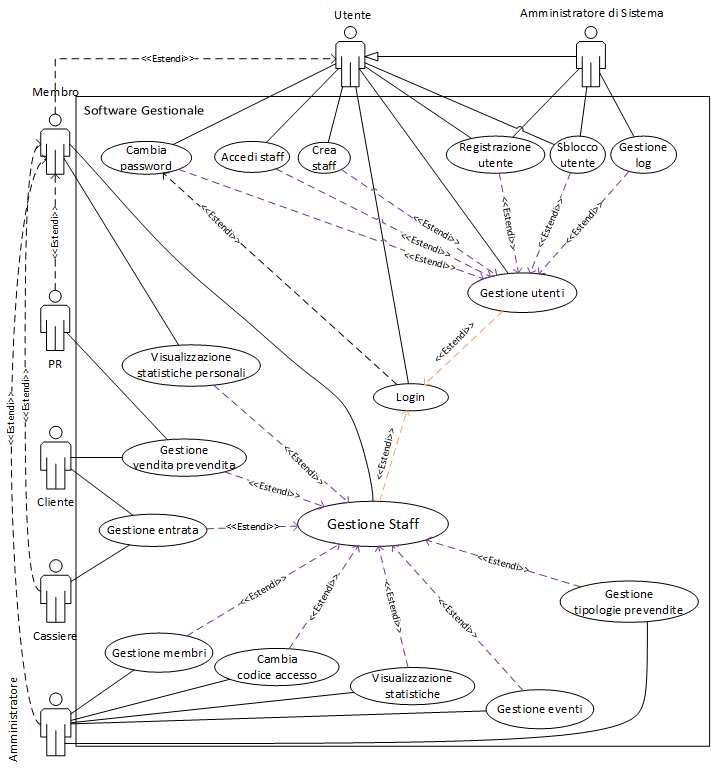
\includegraphics[scale=0.9]{use_cases_aggiornato.png}

Vengono aggiunti due casi d'uso: Gestione log e Sblocco utente. Entrambi casi d'uso sono associati ad un amministratore di sistema.

\newpage

\subsubsection{Scenari aggiornati}

% Gestione log
%Forse da dividere in aggiungi log, leggi log e cancella log.

\begin{center}
\begin{tabularx}{1\textwidth}{|l|X|}
    \hline
	\textbf{Titolo} & Gestione log \\
	\hline
	\textbf{Descrizione} & Gestione del log del software gestionale \\
	\hline
	\textbf{Attori} & Amministratore di sistema \\
	\hline
	\textbf{Relazioni} & Gestione utente \\
	\hline
	\textbf{Precondizioni} &  \\
	\hline
	\textbf{Postcondizioni} &  \\
	\hline
	\textbf{Scenario principale} & 1. L'amministratore di sistema è già autenticato.\\
	                             & 2. L'amministratore di sistema sceglie una funzione: \\
								 & \quad a. Aggiungi log \\
								 & \quad b. Leggi log \\
								 & 3. L'amministratore di sistema esegue l'operazione.\\
								 & 4. Ritorno alla schermata precedente.\\
	\hline
	\textbf{Scenari alternativi} & \\
	\hline
	\textbf{Requisiti non funzionali} & \\
	\hline
	\textbf{Punti aperti} & \\
	\hline
\end{tabularx}
\end{center}

%Sblocco utente

\begin{center}
    \begin{tabularx}{1\textwidth}{|l|X|}
        \hline
        \textbf{Titolo} & Sblocco utente \\
        \hline
        \textbf{Descrizione} & Caso in cui un utente è bloccato e chiede aiuto all'amministratore di sistema. \\
        \hline
        \textbf{Attori} & Amministratore di sistema, Utente \\
        \hline
        \textbf{Relazioni} & Gestione utente \\
        \hline
        \textbf{Precondizioni} &  \\
        \hline
        \textbf{Postcondizioni} &  \\
        \hline
        \textbf{Scenario principale} & 1. L'amministratore di sistema è già autenticato.\\
                                     & 2. L'amministratore si informa riguardo l'utente.\\
                                     & 3. L'utente si spiega di quanto accaduto con l'amministratore.\\
                                     & 4. Se decide di sbloccarlo allora inserisce i dati nell'apposita vista.\\
                                     & 5. L'amministratore esegue l'operazione e l'utente viene sbloccato.\\
        \hline
        \textbf{Scenari alternativi} & \\
        \hline
        \textbf{Requisiti non funzionali} & \\
        \hline
        \textbf{Punti aperti} & \\
        \hline
    \end{tabularx}
\end{center}

Nello scenario login ho aggiunto il requisito non funzionale

\begin{center}
\begin{tabularx}{1\textwidth}{|l|X|}
    \hline
	\textbf{Titolo} & Login \\
	\hline
	\textbf{Descrizione} & Autenticazione nel software gestionale \\
	\hline
	\textbf{Attori} & Utente \\
	\hline
	\textbf{Relazioni} & Cambia Password \\
	\hline
	\textbf{Precondizioni} & L'utente deve essere registato nel sistema \\
	\hline
	\textbf{Postcondizioni} & L'utente è autenticato nel sistema \\
	\hline
	\textbf{Scenario principale} & 1. Impostazione di una schermata per l'inserimento di username e password. \\
								 & 2. L'utente inserisce i dati del proprio account. \\
								 & 3. L'utente esegue l'operazione. \\
								 & 4. Il sistema verifica le credenziali. \\
								 & 5. Dopo l'autenticazione viene mostrata una schermata principale.\\
	\hline
	\textbf{Scenari alternativi} & A) L'utente sbaglia credenziali: \\
								 & \quad 1. Notifica all'utente.\\
								 & \quad 2. Ritorno alla schermata di login.\\
								 & B) L'utente ha sbagliato troppe volte le credenziali: \\
								 & \quad 1. Blocco dell'account.\\
								 & \quad 2. Notifica all'utente.\\
								 & \quad 3. Ritorno alla schermata di login.\\
								 & C) L'utente ha la password di default impostata dall'amministratore di sistema:\\
								 & \quad 1. Passaggio al cambio password.\\
								 & D) L'utente ha l'account bloccato:\\
								 & \quad 1. Notifica all'utente.\\
								 & \quad 2. Ritorno alla schermata di login.\\
								 & E) L'utente è gia autenticato:\\
								 & \quad 1. Mostro la schermata principale.\\
	\hline
	\textbf{Requisiti non funzionali} & \hyperlink{R1NF}{R1NF}, \hyperlink{R6NF}{R6NF}, \hyperlink{R15NF}{R15NF}, \hyperlink{R27NF}{R27NF} \\
	\hline
	\textbf{Punti aperti} & \\
	\hline
\end{tabularx}
\end{center}

\newpage

\subsection{Descrizione delle interfacce grafiche}

%TODO

\newpage

\section{Analisi del problema}

\subsection{Analisi delle funzionalità}

\subsubsection{Tabella delle funzionalità}

\begin{center}
    \begin{tabularx}{1\textwidth}{|X|X|X|X|}
        \hline
        \textbf{Funzionalità} & \textbf{Tipo} & \textbf{Grado di Complessità} & \textbf{Requisiti collegati}\\
        \hline
        \hline
        %Gestione utente & Gestione dei dati, interazione con l'esterno & Complesso & \hyperlink{R7F}{R7F}, \hyperlink{R11F}{R11F}\\
        Gestione utente & Gestione dei dati, memorizzazione dei dati, interazione con l'esterno & Complesso & \\
        \hline
        Gestione log & gestione dei dati, interazione con l'esterno & Semplice & \hyperlink{R26F}{R26F}, \hyperlink{R27F}{R27F}\\
        \hline
        Scrittura log & memorizzazione di dati & Semplice & \hyperlink{R26F}{R26F}\\
        \hline
        Sblocco utente & Gestione dei dati, memorizzazione di dati, interazione con l'esterno & Semplice & \hyperlink{R28F}{R28F}\\
        \hline
        Registrazione utente & Gestione dei dati, memorizzazione di dati, interazione con l'esterno & Complesso & \hyperlink{R2F}{R2F}, \hyperlink{R3F}{R3F}, \hyperlink{R5F}{R5F} \\
        \hline
        Crea staff & Gestione dei dati, memorizzazione di dati, interazione con l'esterno & Complesso & \hyperlink{R1F}{R1F}, \hyperlink{R4F}{R4F}, \hyperlink{R12F}{R12F}\\
        \hline
        Accedi staff & Gestione dei dati, memorizzazione di dati, interazione con l'esterno & Semplice & \hyperlink{R1F}{R1F}, \hyperlink{R4F}{R4F}, \hyperlink{R11F}{R11F} \\
        \hline
        Cambia password & Gestione dei dati, interazione con l'esterno & Semplice & \hyperlink{R3F}{R3F}, \hyperlink{R6F}{R6F} \\
        \hline
        %Gestione staff & Gestione dei dati, interazione con l'esterno & Complesso & \hyperlink{R7F}{R7F}, \hyperlink{R10F}{R10F},  \\
        Gestione staff & Gestione dei dati, memorizzazione dei dati, interazione con l'esterno & Complesso &  \\
        \hline
        Visualizzazione statistiche personali & Lettura dati, interazione con l'esterno & Semplice &  \hyperlink{R24F}{R24F} \\
        \hline
        Gestione vendita prevendita & Gestione dei dati, memorizzazione di dati, interazione con l'esterno & Complesso & \hyperlink{R9F}{R9F}, \hyperlink{R14F}{R14F}, \hyperlink{R15F}{R15F}, \hyperlink{R23F}{R23F}, \hyperlink{R25F}{R25F} \\
        \hline
        Gestione entrata & Gestione dei dati, memorizzazione di dati, interazione con l'esterno & Complesso & \hyperlink{R8F}{R8F}, \hyperlink{R13F}{R13F}, \hyperlink{R14F}{R14F} \\
        \hline
        Gestione membri & Gestione dei dati, interazione con l'esterno & Complesso & \hyperlink{R7F}{R7F}, \hyperlink{R10F}{R10F}, \hyperlink{R16F/NF}{R16F/NF} \\
        \hline
        Cambia codice accesso & Gestione dei dati, interazione con l'esterno & Semplice & \hyperlink{R17F}{R17F}  \\
        \hline
        Visualizzazione statistiche & Lettura dati, interazione con l'esterno & Semplice & \hyperlink{R10F}{R10F}  \\
        \hline
        Gestione eventi & Gestione dei dati, memorizzazione di dati, interazione con l'esterno & Complesso & \hyperlink{R10F}{R10F}, \hyperlink{R18F}{R18F}, \hyperlink{R20F}{R20F}, \hyperlink{R21F}{R21F} \\
        \hline
        Gestione tipologie prevendite & Gestione dei dati, memorizzazione di dati, interazione con l'esterno & Complesso & \hyperlink{R10F}{R10F}, \hyperlink{R19F}{R19F}, \hyperlink{R22F}{R22F} \\
        \hline
        Autenticazione & Lettura di dati, interazione con l'esterno & Semplice & \hyperlink{R2F}{R2F}, \hyperlink{R3F}{R3F} \\
        \hline
    \end{tabularx}
\end{center}

\newpage

\subsubsection{Tabelle Informazioni/Flusso}

\textbf{Gestione Utente - Tabella Informazioni/Flusso}

\begin{center}
    \begin{tabularx}{1\textwidth}{|X|X|X|X|X|}
        \hline
        \textbf{Informazione} &\textbf{Tipo} & \textbf{Livello protezione / Privacy} & \textbf{Input/Output} & \textbf{Vincoli}\\
        \hline
        \hline
        %Da chiedere se da mettere
        %Tipologia utente & Semplice & Alto & Input & Enumeratore: Utente normale o Amministratore di sistema \\
        \hline
    \end{tabularx}
\end{center}

\textbf{Gestione log  - Tabella Informazioni/Flusso}

\begin{center}
    \begin{tabularx}{1\textwidth}{|X|X|X|X|X|}
        \hline
        \textbf{Informazione} &\textbf{Tipo} & \textbf{Livello protezione / Privacy} & \textbf{Input/Output} & \textbf{Vincoli}\\
        \hline
        \hline
        Record d'inserimento & Complesso & Medio & Input & \\
        \hline
        Record di lettura & Complesso & Medio & Output & \\
        \hline
    \end{tabularx}
\end{center}

\textbf{Scrittura log  - Tabella Informazioni/Flusso}

\begin{center}
    \begin{tabularx}{1\textwidth}{|X|X|X|X|X|}
        \hline
        \textbf{Informazione} &\textbf{Tipo} & \textbf{Livello protezione / Privacy} & \textbf{Input/Output} & \textbf{Vincoli}\\
        \hline
        \hline
        Timestamp record & Semplice & Medio & Input & \\
        \hline
        Descrizione record & Semplice & Medio & Input & Non più di 256 caratteri \\
        \hline
        Livello di importanza record & Semplice & Medio & Input & Enumeratore: Basso, Medio, Alto\\
        \hline
    \end{tabularx}
\end{center}

\textbf{Sblocco utente  - Tabella Informazioni/Flusso}

\begin{center}
    \begin{tabularx}{1\textwidth}{|X|X|X|X|X|}
        \hline
        \textbf{Informazione} &\textbf{Tipo} & \textbf{Livello protezione / Privacy} & \textbf{Input/Output} & \textbf{Vincoli}\\
        \hline
        \hline
        Informazioni per lo sblocco & Complesso & Medio & Input & \\
        \hline
    \end{tabularx}
\end{center}

\textbf{Registrazione utente  - Tabella Informazioni/Flusso}

\begin{center}
    \begin{tabularx}{1\textwidth}{|X|X|X|X|X|}
        \hline
        \textbf{Informazione} &\textbf{Tipo} & \textbf{Livello protezione / Privacy} & \textbf{Input/Output} & \textbf{Vincoli}\\
        \hline
        \hline
        Nome & Semplice & Medio & Input & Non più di 100 caratteri\\
        \hline
        Cognome & Semplice & Medio & Input & Non più di 100 caratteri\\
        \hline
        Telefono & Semplice & Alto & Input & Non più di 20 caratteri\\
        \hline
        Username & Semplice & Alto & Input & Non più di 20 caratteri\\
        \hline
        Password & Semplice & Alto & Input & \hyperlink{R1NF}{R1NF}, non più di 50 caratteri\\
        \hline
    \end{tabularx}
\end{center}

\textbf{Crea staff  - Tabella Informazioni/Flusso}

\begin{center}
    \begin{tabularx}{1\textwidth}{|X|X|X|X|X|}
        \hline
        \textbf{Informazione} &\textbf{Tipo} & \textbf{Livello protezione / Privacy} & \textbf{Input/Output} & \textbf{Vincoli}\\
        \hline
        \hline
        Nome & Semplice & Basso & Input & Non più di 100 caratteri\\
        \hline
        Codice di accesso & Semplice & Alto & Input & \hyperlink{R2NF}{R2NF}, Non più di 50 caratteri\\
        \hline
    \end{tabularx}
\end{center}

\textbf{Accedi staff  - Tabella Informazioni/Flusso}

\begin{center}
    \begin{tabularx}{1\textwidth}{|X|X|X|X|X|}
        \hline
        \textbf{Informazione} &\textbf{Tipo} & \textbf{Livello protezione / Privacy} & \textbf{Input/Output} & \textbf{Vincoli}\\
        \hline
        \hline
        Nome & Semplice & Basso & Input & Non più di 100 caratteri\\
        \hline
        Codice di accesso & Semplice & Alto & Input & \hyperlink{R2NF}{R2NF}, Non più di 50 caratteri\\
        \hline
    \end{tabularx}
\end{center}

\textbf{Cambia password  - Tabella Informazioni/Flusso}

\begin{center}
    \begin{tabularx}{1\textwidth}{|X|X|X|X|X|}
        \hline
        \textbf{Informazione} &\textbf{Tipo} & \textbf{Livello protezione / Privacy} & \textbf{Input/Output} & \textbf{Vincoli}\\
        \hline
        \hline
        Vecchia password & Semplice & Alto & Input & \hyperlink{R1NF}{R1NF}, Non più di 50 caratteri\\
        \hline
        Nuova password & Semplice & Alto & Input & \hyperlink{R1NF}{R1NF}, Non più di 50 caratteri\\
        \hline
    \end{tabularx}
\end{center}

\textbf{Gestione staff  - Tabella Informazioni/Flusso}

\begin{center}
    \begin{tabularx}{1\textwidth}{|X|X|X|X|X|}
        \hline
        \textbf{Informazione} &\textbf{Tipo} & \textbf{Livello protezione / Privacy} & \textbf{Input/Output} & \textbf{Vincoli}\\
        \hline
        \hline
        %Ruolo & Semplce & Alto & Input & \hyperlink{R7F}{R7F} \\
    \end{tabularx}
\end{center}

\textbf{Visualizzazione statistiche personali  - Tabella Informazioni/Flusso}

\begin{center}
    \begin{tabularx}{1\textwidth}{|X|X|X|X|X|}
        \hline
        \textbf{Informazione} &\textbf{Tipo} & \textbf{Livello protezione / Privacy} & \textbf{Input/Output} & \textbf{Vincoli}\\
        \hline
        \hline
        Entrate svolte & Complesso & Basso & Output & \\
        \hline
        Guadagni & Complesso & Basso & Output & \\
        \hline
    \end{tabularx}
\end{center}

\textbf{Gestione vendita prevendita  - Tabella Informazioni/Flusso}

\begin{center}
    \begin{tabularx}{1\textwidth}{|X|X|X|X|X|}
        \hline
        \textbf{Informazione} &\textbf{Tipo} & \textbf{Livello protezione / Privacy} & \textbf{Input/Output} & \textbf{Vincoli}\\
        \hline
        \hline
        Informazioni base cliente & Complesso & Medio & Input & \hyperlink{R25F}{R25F}\\
        \hline
        Prevendita & Complesso & Medio & Input & \hyperlink{R25F}{R25F}, \hyperlink{R8NF}{R8NF}, \hyperlink{R9NF}{R9NF}, \hyperlink{R13NF}{R13NF}, \hyperlink{R14NF}{R14NF}, \hyperlink{R16NF}{R16NF}, \hyperlink{R18NF}{R18NF}, \hyperlink{R26NF}{R26NF} \\
        \hline
        Documento digitale & Complesso & Medio & Output & \hyperlink{R11NF}{R11NF}, \hyperlink{R26NF}{R26NF}  \\
        \hline
    \end{tabularx}
\end{center}

\textbf{Gestione entrata  - Tabella Informazioni/Flusso}

\begin{center}
    \begin{tabularx}{1\textwidth}{|X|X|X|X|X|}
        \hline
        \textbf{Informazione} &\textbf{Tipo} & \textbf{Livello protezione / Privacy} & \textbf{Input/Output} & \textbf{Vincoli}\\
        \hline
        \hline
        Informazioni base cliente & Complesso & Medio & Input & \hyperlink{R25F}{R25F}\\
        \hline
        Documento digitale & Complesso & Medio & Input & \hyperlink{R11NF}{R11NF}, \hyperlink{R26NF}{R26NF}  \\
        \hline
        Prevendita & Complesso & Medio & Output & \\
        \hline
    \end{tabularx}
\end{center}

\textbf{Gestione membri  - Tabella Informazioni/Flusso}

\begin{center}
    \begin{tabularx}{1\textwidth}{|X|X|X|X|X|}
        \hline
        \textbf{Informazione} &\textbf{Tipo} & \textbf{Livello protezione / Privacy} & \textbf{Input/Output} & \textbf{Vincoli}\\
        \hline
        \hline
        Informazioni membro & Complesso & Alto & Input & \hyperlink{R7F}{R7F}\\
        \hline
    \end{tabularx}
\end{center}


\textbf{Cambia codice accesso  - Tabella Informazioni/Flusso}

\begin{center}
    \begin{tabularx}{1\textwidth}{|X|X|X|X|X|}
        \hline
        \textbf{Informazione} &\textbf{Tipo} & \textbf{Livello protezione / Privacy} & \textbf{Input/Output} & \textbf{Vincoli}\\
        \hline
        \hline
        Nome dello staff & Semplice & Basso & Input & \\
        \hline
        Vecchio codice di accesso & Semplice & Alto & Input & \hyperlink{R2NF}{R2NF}, Non più di 50 caratteri\\
        \hline
        Nuovo codice di accesso & Semplice & Alto & Input & \hyperlink{R2NF}{R2NF}, Non più di 50 caratteri\\
        \hline
        \hline
    \end{tabularx}
\end{center}

\textbf{Visualizzazione statistiche  - Tabella Informazioni/Flusso}

\begin{center}
    \begin{tabularx}{1\textwidth}{|X|X|X|X|X|}
        \hline
        \textbf{Informazione} &\textbf{Tipo} & \textbf{Livello protezione / Privacy} & \textbf{Input/Output} & \textbf{Vincoli}\\
        \hline
        \hline
        Entrate evento & Complesso & Basso & Output & \\
        \hline
        Guadagni evento & Complesso & Basso & Output & \\
        \hline
        Entrate membro & Complesso & Basso & Output & \\
        \hline
        Guadagni membro & Complesso & Basso & Output & \\
        \hline
        \hline
    \end{tabularx}
\end{center}

\textbf{Gestione eventi  - Tabella Informazioni/Flusso}

\begin{center}
    \begin{tabularx}{1\textwidth}{|X|X|X|X|X|}
        \hline
        \textbf{Informazione} &\textbf{Tipo} & \textbf{Livello protezione / Privacy} & \textbf{Input/Output} & \textbf{Vincoli}\\
        \hline
        \hline
        Evento & Complesso & Medio & Input & \hyperlink{R20F}{R20F}, \hyperlink{R21F}{R21F} \\
        \hline
    \end{tabularx}
\end{center}

\textbf{Gestione tipologie prevendite  - Tabella Informazioni/Flusso}

\begin{center}
    \begin{tabularx}{1\textwidth}{|X|X|X|X|X|}
        \hline
        \textbf{Informazione} &\textbf{Tipo} & \textbf{Livello protezione / Privacy} & \textbf{Input/Output} & \textbf{Vincoli}\\
        \hline
        \hline
        Tipologia prevendita & Complesso & Alto & Input & \hyperlink{R22F}{R22F} \\
        \hline
    \end{tabularx}
\end{center}

\textbf{Autenticazione  - Tabella Informazioni/Flusso}

\begin{center}
    \begin{tabularx}{1\textwidth}{|X|X|X|X|X|}
        \hline
        \textbf{Informazione} &\textbf{Tipo} & \textbf{Livello protezione / Privacy} & \textbf{Input/Output} & \textbf{Vincoli}\\
        \hline
        \hline
        Username & Semplice & Alto & Input & Non più di 20 caratteri\\
        \hline
        Password & Semplice & Alto & Input & \hyperlink{R1NF}{R1NF}, non più di 50 caratteri\\
        \hline
    \end{tabularx}
\end{center}

\subsection{Analisi dei vincoli}
\subsubsection{Tabella dei vincoli}


%\hyperlink{R21NF}{R21NF} I dati della comunicazione devono essere protetti.
%\hyperlink{R22NF}{R22NF} I dati persistenti devono essere protetti
%\hyperlink{R23NF}{R23NF} Il sistema deve verificare le autorizzazioni degli utenti e dei membri.

\begin{center}
    \begin{tabularx}{1\textwidth}{|X|X|X|X|}
    \hline
    \textbf{Requisito} & \textbf{Categoria} & \textbf{Impatto} & \textbf{Funzionalità}\\
    \hline
    \hline
    Facile navigabilità delle schermate (\hyperlink{R20NF}{R20NF} & Usabilità & Cercare di migliorare & Gestione vendite prevendita,  Gestione entrata, Autenticazione\\
    \hline
    Protezione dei dati (\hyperlink{R21NF}{R21NF}, \hyperlink{R22NF}{R22NF}) & Sicurezza & Peggiorano tempo di risposta, migliorano la privacy dei dati & Gestione log, Scrittura log, Sblocco utente, Registrazione utente, Crea staff, Accedi staff, Cambia password, Visualizzazione statistiche personali, Gestione vendita prevendita, Gestione entrata, Gestione membri, Cambia codice accesso, Visualizzazione statistiche, Gestione eventi, Gestione tipologie prevendite, Autenticazione\\
    \hline
    Controllo accessi (\hyperlink{R23NF}{R23NF}) & Sicurezza & Peggiorano tempo di risposta e usabilità, migliorano la privacy dei dati & Gestione utente, Gestione staff\\
    \hline
    \end{tabularx}
\end{center}

\newpage

\subsection{Analisi delle interazioni}
\subsubsection{Tabella delle maschere}

\begin{center}
    \begin{tabularx}{1\textwidth}{|X|X|X|X|}
    \hline
    \textbf{Maschera} & \textbf{Informazioni} & \textbf{Funzionalità}\\
    \hline
    \hline
    View Autenticazione & username, password & Autenticazione\\
    \hline
    Home Gestione utente & navigabilità delle funzioni utente e amministratore di sistema & Gestione utente\\
    \hline
    Home Gestione log & navigabilità delle funzioni gestione log: aggiungi log e leggi log & Gestione log\\
    \hline
    View Aggiungi log & timestamp, descrizione, livello & Gestione log\\
    \hline
    View Leggi log & timestamp, descrizione, livello & Gestione log\\
    \hline
    View Sblocco utente & dati utente da sbloccare & Sblocco utente \\
    \hline
    View Registrazione utente & nome, cognome, telefono, username, password & Registrazione utente\\
    \hline
    View Crea staff & nome, codice di accesso & Crea staff\\
    \hline
    View Accedi staff & nome, codice di accesso & Accedi staff\\
    \hline
    View Cambia password & vecchia password, nuova password & Cambia password\\
    \hline
    Home Gestione staff & consente la navigabilità delle funzioni del membro, PR, cassiere e amministratore & Gestione staff\\
    \hline
    View Visualizzazione statistiche personali & entrate svolte, guadagni, filtri dei dati per evento, staff e totale & Visualizzazione statistiche personali\\
    \hline
    Home Gestione vendita prevendita & navigabilità tra le funzioni del PR & Gestione vendita prevendita\\
    \hline
    View Aggiungi prevendita & informazioni cliente, evento prevendita, tipologia prenvendita, documento finale & Gestione vendita prevendita\\
    \hline
    View Lista prevendite & informazioni cliente, evento e tipologia, filtri in base al cliente e all'evento & Gestione vendita prevendita\\
    \hline
    View Annulla prevendita & informazioni prevendita per l'annullamento & Gestionve vendita prevendita\\
    \hline
    Home Gestione entrata & fornisce la navigabilità tra le funzioni del Cassiere & Gestione entrata\\
    \hline
    View Timbra entrata & documento digitale & Gestione entrata\\
    \hline
    View Lista entrate & entrata, filtri per evento, staff & Gestione entrata\\
    \hline
    Home gestione membri & fornisce la navigabilità tra le funzioni di gestione dei membri da parte dell'amministratore & Gestione membri\\
    \hline
    View lista membri & informazioni sui membri & Gestione membri\\
    \hline
    View Modifica ruoli membro & informazioni del membro da modficare, nuovi ruoli & Gestione membri\\
    \hline
    View Rimuovi membro & informazioni del membro da eliminare & Gestione membri\\
    \hline
    View Cambia codice di accesso & nome staff, vecchio codice, nuovo codice & Cambia codice accesso\\
    \hline
    View Visualizzazione statistiche & informazioni membro, entrate effettuate, guadagni, informazioni evento, entrate evento, guadagni evento, filtro per membro o per evento & Visualizzazione statistiche\\
    \hline
    \end{tabularx}
\end{center}

\begin{center}
    \begin{tabularx}{1\textwidth}{|X|X|X|X|}
    \hline
    \textbf{Maschera} & \textbf{Informazioni} & \textbf{Funzionalità}\\
    \hline
    \hline
    Home Gestione eventi & fornisce la navigabilità tra le funzioni di gestione eventi da parte dell'amministratore & Gestione eventi \\
    \hline
    View Aggiungi evento & nome, descrizione, periodo temporale e luogo di svolgimento & Gestione eventi\\
    \hline
    View Lista eventi & nome, descrizione, periodo temporale e luogo di svolgimento & Gestione eventi\\
    \hline
    View Modifica evento & informazioni dell'evento da modificare, modifiche da effettuare & Gestione eventi\\
    \hline
    View Annulla evento & informazioni dell'evento da annullare & Gestione eventi\\
    \hline
    Home Gestione tipologie prevendite & fornisce la navigabilità tra le funzioni di gestione tipologie prevendite da parte dell'amministratore & Gestione tipologie prevendite \\
    \hline
    View Aggiungi tipologia prevendita & nome, descrizione, periodo temporale di vendita e prezzo & Gestione tipologie prevendite\\
    \hline
    View Lista tipologie prevendite & nome, descrizione, periodo temporale di vendita e prezzo & Gestione tipologie prevendite\\
    View Modifica tipologia prevendita & informazioni della tipologia prevendita da modificare, modifiche da effettuare & Gestione tipologie prevendite\\
    \hline
    View Elimina tipologia prevendita & informazioni della tipologia prevendita da eliminare & Gestione tipologie prevendite\\
    \hline
    \end{tabularx}
\end{center}

\newpage

\subsection{Analisi dei ruoli e responsabilità}
\subsubsection{Tabella dei ruoli}


\begin{center}
    \begin{tabularx}{1\textwidth}{|X|X|X|X|X|X|}
    \hline
    \textbf{Ruolo} & \textbf{Responsabilità} & \mc{2}{\textbf{Maschere}} & \textbf{Riservatezza} & \textbf{Numerosità}\\
    \hline
    \hline
    Utente & Può creare uno staff, e accedere ad altri staff. & \mc{2}{View Autenticazione, Home Gestione utente, View Crea staff, View Accedi staff, View Cambia password} & Alto grado di riservatezza & Il numero può essere gestito dall'amministratore di sistema, al più è limitato dalle risorse del sistema \\ 
    \hline
    Amministratore di sistema & Può fare tutte le operazioni di un utente e in più gestisce il log, lo sblocco di utenti bloccati e la registrazione di un nuovo utente & \mc{2}{View Autenticazione, Home Gestione utente, View Crea staff, View Accedi staff, View Cambia password, Home gestione log, View Aggiungi log, View Leggi Log, View Sblocco utente, View Registrazione utente} & Massimo grado di riservatezza & per ogni installazione software è sufficiente un amministratore di sistema\\
    \hline
    Membro di uno staff & Può ricavare informazioni sullo staff, può leggere le statistiche ad esso attribuite. & \mc{2}{Home gestione staff, View Visualizzazione statistiche personali} & Alto grado di riservatezza & Numero massimo limitato dalle risorse del sistema \\
    \hline
    Cassiere di uno staff & Può effettuare tutte le operazioni di un membro e in più gestisce le entrate di un evento. & \mc{2}{Home gestione staff, View Visualizzazione statistiche personali, Home Gestione entrata, View Timbra entrata, View lista entrate} & Alto grado di riservatezza & Numero massimo limitato dalle risorse del sistema\\
    \hline
    PR di uno staff & Può effettuare tutte le operazioni di un membro e in più gestisce la vendita di prevendite & \mc{2}{Home gestione staff, View Visualizzazione statistiche personali, Home Gestione vendita prevendita, View Aggiungi prevendita, View Lista prevendite, View Annulla prevendita} & Alto grado di riservatezza & Numero massimo limitato dalle risorse del sistema\\
    \hline
    Amministratore di uno staff & Può effettuare tutte le operazioni di un membro e in più gestisce lo staff & \mc{2}{Home gestione staff, View Visualizzazione statistiche personali, Home Gestione membri, View lista membri, View Modifica ruoli membro, View Rimuovi membro, View Cambia codice di accesso, View Visualizzazione statistiche, Home Gestione eventi, View Aggiungi evento, View lista eventi, View Modifica evento, View Annulla evento, Home gestione tipologie prevendite, View Aggiungi tipologia prevendita, View lista tipologie prevendite, View modifica tipologia prevendita, View elimina tipologia prevendita} & Alto grado di riservatezza & Numero massimo limitato dalle risorse del sistema\\
    \hline
    \end{tabularx}
\end{center}

\newpage

\subsubsection{Tabelle Ruolo-Informazioni}

\textbf{Utente: Tabella Ruolo-Informazioni}

\begin{center}
    \begin{tabularx}{1\textwidth}{|X|X|}
    \hline
    \textbf{Informazione} & \textbf{Tipo di accesso} \\
    \hline
    \hline
    Dati personali & Lettura\\
    \hline
    Password personale & Scrittura\\
    \hline
    Staff & Lettura/Scrittura\\
    \hline
    \end{tabularx}
\end{center}

\textbf{Amministratore di sistema: Tabella Ruolo-Informazioni}

\begin{center}
    \begin{tabularx}{1\textwidth}{|X|X|}
    \hline
    \textbf{Informazione} & \textbf{Tipo di accesso} \\
    \hline
    \hline
    Dati personali & Lettura\\
    \hline
    Password personale & Scrittura\\
    \hline
    Staff & Lettura/Scrittura\\
    \hline
    Utente & Lettura/Scrittura\\
    \hline
    Log & Lettura/Scrittura\\
    \hline
    \end{tabularx}
\end{center}

\textbf{Membro di uno staff: Tabella Ruolo-Informazioni}

\begin{center}
    \begin{tabularx}{1\textwidth}{|X|X|}
    \hline
    \textbf{Informazione} & \textbf{Tipo di accesso} \\
    \hline
    \hline
    Dati personali & Lettura\\
    \hline
    Informazioni sullo staff & Lettura\\
    \hline
    Statistiche personali & Lettura\\
    \hline
    \end{tabularx}
\end{center}

\textbf{Cassiere staff: Tabella Ruolo-Informazioni}

\begin{center}
    \begin{tabularx}{1\textwidth}{|X|X|}
    \hline
    \textbf{Informazione} & \textbf{Tipo di accesso} \\
    \hline
    \hline
    Dati personali & Lettura\\
    \hline
    Informazioni sullo staff & Lettura\\
    \hline
    Statistiche personali & Lettura\\
    \hline
    Prevendite & Lettura\\
    \hline
    Entrate & Lettura/Scrittura\\
    \hline
    Tipologie prevendita & Lettura\\
    \hline
    Evento & Lettura\\
    \hline
    \end{tabularx}
\end{center}

\textbf{PR di uno staff: Tabella Ruolo-Informazioni}

\begin{center}
    \begin{tabularx}{1\textwidth}{|X|X|}
    \hline
    \textbf{Informazione} & \textbf{Tipo di accesso} \\
    \hline
    \hline
    Dati personali & Lettura\\
    \hline
    Informazioni sullo staff & Lettura\\
    \hline
    Statistiche personali & Lettura\\
    \hline
    Prevendite & Lettura/Scrittura\\
    \hline
    Tipologie prevendita & Lettura\\
    \hline
    Evento & Lettura\\
    \hline
    \end{tabularx}
\end{center}

\textbf{Amministratore di uno staff: Tabella Ruolo-Informazioni}

\begin{center}
    \begin{tabularx}{1\textwidth}{|X|X|}
    \hline
    \textbf{Informazione} & \textbf{Tipo di accesso} \\
    \hline
    \hline
    Dati personali & Lettura\\
    \hline
    Informazioni sullo staff & Lettura\\
    \hline
    Statistiche personali & Lettura\\
    \hline
    Evento & Lettura/Scrittura\\
    \hline
    Tipologie Prevendite & Lettura/Scrittura\\
    \hline
    Statistiche & Lettura\\
    \hline
    Codice di accesso & Scrittura\\
    \hline
    Membri dello staff & Lettura/Scrittura\\
    \hline
    Ruoli di un membro & Lettura/Scrittura\\
    \hline
    \end{tabularx}
\end{center}

\newpage

\subsection{Scomposizione del problema}

\begin{center}
    \begin{tabularx}{1\textwidth}{|X|X|}
    \hline
    \textbf{Funzionalità} & \textbf{Scomposizione} \\
    \hline
    \hline
    Gestione utente & Crea staff, Accedi staff, Cambia password, Gestione log, Sblocco utente, Registrazione utente\\
    \hline
    Gestione log & Leggi log, Aggiungi log\\
    \hline
    Gestione staff & Visualizzazione statistiche personali, Gestione vendita prevendita, Gestione entrata, Gestione membri, Cambia codice accesso, Visualizzazione statistiche, Gestione eventi, Gestione tipologie prevendita\\
    \hline
    Gestione vendita prevendita & Aggiungi prevendita, Lista prevendite, Annulla prevendita\\
    \hline
    Gestione entrata & Timbra entrata, Lista entrate\\
    \hline
    Gestione membri & Lista membri, Modifica ruoli membro, Rimuovi membro\\
    \hline
    Gestione eventi & Aggiungi evento, Lista eventi, Modifica evento, Annulla evento\\
    \hline
    Gestione tipologie prevendita & Aggiungi tipologia prevendita, Lista tipologie prevendita, Modifica tipologia prevendita, Rimuovi tipologia prevendita\\
    \hline
    \end{tabularx}
\end{center}


\textbf{Gestione utente: Tabella Sotto-Funzionalità}

\begin{center}
    \begin{tabularx}{1\textwidth}{|X|X|X|X|}
    \hline
    \textbf{Sotto-funzionalità} & \textbf{Sotto-funzionalità} & \textbf{Legame} & \textbf{Informazioni}\\
    \hline
    \hline
    Registrazione utente & Sblocco utente & Si può sbloccare un utente solo se è registrato & username\\
    \hline
    Crea staff & Accedi staff & Si può accedere ad uno staff solo se è stato creato & nome staff\\
    \hline
    \end{tabularx}
\end{center}

\textbf{Gestione log: Tabella Sotto-Funzionalità}

\begin{center}
    \begin{tabularx}{1\textwidth}{|X|X|X|X|}
    \hline
    \textbf{Sotto-funzionalità} & \textbf{Sotto-funzionalità} & \textbf{Legame} & \textbf{Informazioni}\\
    \hline
    \hline
    Aggiungi log & Leggi log & Si può leggere un record solo se è stato aggiunto & record\\
    \hline
    \end{tabularx}
\end{center}

\textbf{Gestione staff: Tabella Sotto-Funzionalità}

\begin{center}
    \begin{tabularx}{1\textwidth}{|X|X|X|X|}
    \hline
    \textbf{Sotto-funzionalità} & \textbf{Sotto-funzionalità} & \textbf{Legame} & \textbf{Informazioni}\\
    \hline
    \hline
    Gestione vendita prevendita & Gestione eventi & La gestione vendita prevendita deve poter leggere gli eventi per inserirlo nella prevendita & eventi\\
    \hline
    Gestione vendita prevendita & Gestione tipologie prevendita & La gestione vendita prevendita deve poter leggere le tipologie prevendita per l'associazione alla prevendita & tipologie prevendita\\
    \hline
    Gestione vendita prevendita & Gestione entrata & Non posso annullare una prevendita se è già stata usata & prevendita\\
    \hline
    Gestione tipologie prevendita & Gestione eventi & Non posso creare una tipologia prevendita con un periodo di vendita durante o dopo l'evento (\hyperlink{R8NF}{R8NF}) & evento\\
    \hline
    \end{tabularx}
\end{center}

\textbf{Gestione vendita prevendita: Tabella Sotto-Funzionalità}

\begin{center}
    \begin{tabularx}{1\textwidth}{|X|X|X|X|}
    \hline
    \textbf{Sotto-funzionalità} & \textbf{Sotto-funzionalità} & \textbf{Legame} & \textbf{Informazioni}\\
    \hline
    \hline
    Aggiungi prevendita & Lista prevendite & La lista delle prevendite è condizionata dalle prevendite aggiunte & prevendita\\
    \hline
    Aggiungi prevendita & Annulla prevendita & Si può annullare una prevendita solo se è stata aggiunta & prevendita\\
    \hline
    \end{tabularx}
\end{center}

\textbf{Gestione entrata: Tabella Sotto-Funzionalità}

\begin{center}
    \begin{tabularx}{1\textwidth}{|X|X|X|X|}
    \hline
    \textbf{Sotto-funzionalità} & \textbf{Sotto-funzionalità} & \textbf{Legame} & \textbf{Informazioni}\\
    \hline
    \hline
    Timbra Entrata & Lista entrate & La lista delle entrate è condizionata dalle entrate aggiunte & entrata\\
    \hline
    \end{tabularx}
\end{center}

\textbf{Gestione membri: Tabella Sotto-Funzionalità}

\begin{center}
    \begin{tabularx}{1\textwidth}{|X|X|X|X|}
    \hline
    \textbf{Sotto-funzionalità} & \textbf{Sotto-funzionalità} & \textbf{Legame} & \textbf{Informazioni}\\
    \hline
    \hline
    Lista membri & Rimuovi membro & Posso eliminare un membro solo se fa parte della lista, cioè dello staff & membro\\
    \hline
    \end{tabularx}
\end{center}

\textbf{Gestione eventi: Tabella Sotto-Funzionalità}

\begin{center}
    \begin{tabularx}{1\textwidth}{|X|X|X|X|}
    \hline
    \textbf{Sotto-funzionalità} & \textbf{Sotto-funzionalità} & \textbf{Legame} & \textbf{Informazioni}\\
    \hline
    \hline
    Aggiungi evento & Lista eventi & La lista delle prevendite è condizionata dalle prevendite aggiunte & prevendita\\
    \hline
    Aggiungi prevendita & Annulla prevendita & Si può annullare una prevendita solo se è stata aggiunta & prevendita\\
    \hline
    \end{tabularx}
\end{center}

\textbf{Gestione tipologie prevendita: Tabella Sotto-Funzionalità}

\begin{center}
    \begin{tabularx}{1\textwidth}{|X|X|X|X|}
    \hline
    \textbf{Sotto-funzionalità} & \textbf{Sotto-funzionalità} & \textbf{Legame} & \textbf{Informazioni}\\
    \hline
    \hline
    Aggiungi tipologia prevendita & Lista tipologie prevendita & La lista delle tipologie prevendita è condizionata dalle tipologie prevendita aggiunte & tipologia prevendita\\
    \hline
    Aggiungi tipologie prevendita & Annulla tipologie prevendita & Si può annullare una tipologie prevendita solo se è stata aggiunta & tipologia prevendita\\
    \hline
    \end{tabularx}
\end{center}

\newpage

\subsection{Creazione del modello del dominio}

Analizzando il vocabolario si evidenzia il privilegio dell'utente che può essere normale o amministratore di sistema, i ruoli di un membro che possono essere cassiere, pr o amministratore.\\Dall'analisi del vocabolario, rivisto dopo l'analisi di sicurezza, si evidenzia anche il log, con i livelli di importanza: basso, medio, alto.\\\textbf{Qui sotto il modello del dominio:}\\

%TODO: Chiedere al prof se i versi delle molteplicità vanno bene   
%TODO: Chiedere anche per le operazioni

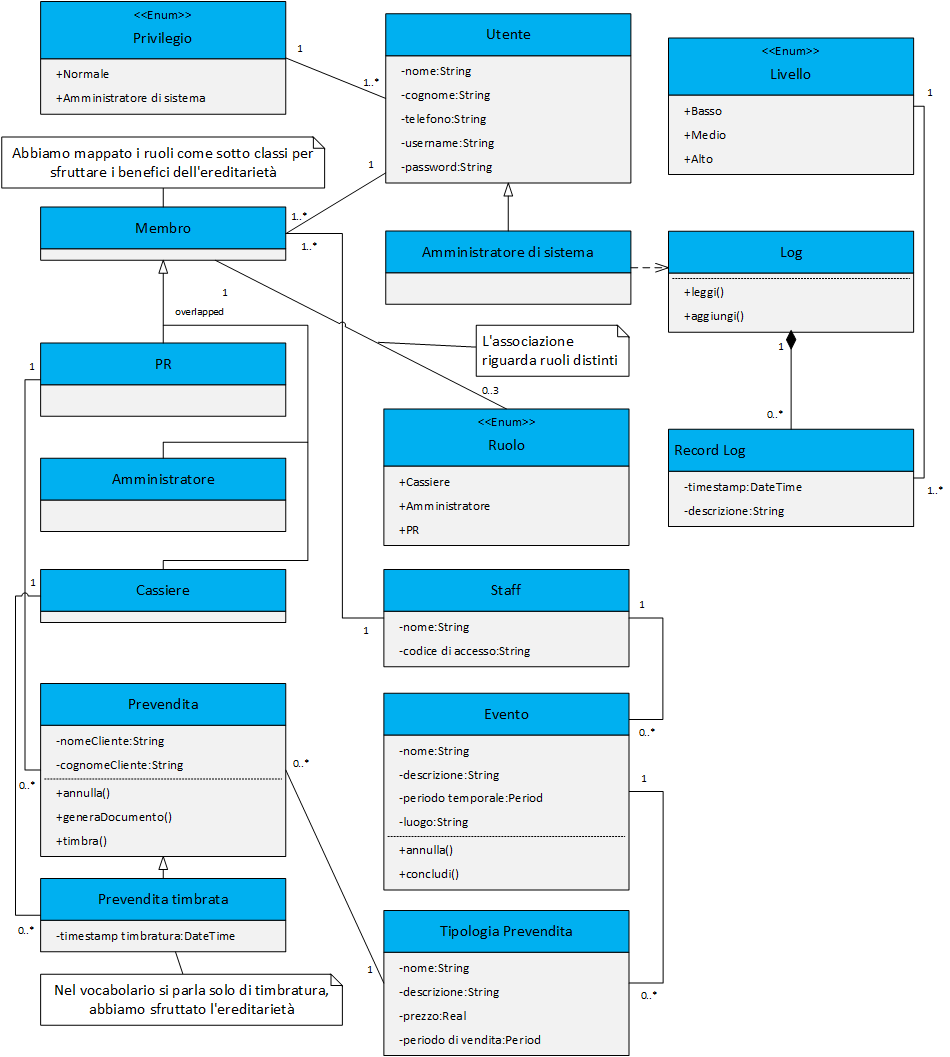
\includegraphics[scale=0.68]{modello_dominio.png}

\newpage

\subsection{Architettura logica}



\end{document}
